\documentclass[a4paper, 12pt]{article}
\usepackage[utf8]{inputenc}
\usepackage[english, ukrainian]{babel}

\usepackage{amsmath, amssymb}
\usepackage{multicol}
\usepackage{graphicx}
\usepackage{float}

\allowdisplaybreaks
\setlength\parindent{0pt}
\numberwithin{equation}{subsection}

\usepackage{hyperref}
\hypersetup{unicode=true,colorlinks=true,linktoc=all,linkcolor=red}

\numberwithin{equation}{subsection}

\renewcommand{\bf}[1]{\textbf{#1}}
\renewcommand{\it}[1]{\textit{#1}}
\newcommand{\bb}[1]{\mathbb{#1}}
\renewcommand{\cal}[1]{\mathcal{#1}}

\renewcommand{\epsilon}{\varepsilon}
\renewcommand{\phi}{\varphi}

\DeclareMathOperator{\diam}{diam}
\DeclareMathOperator{\rang}{rang}
\DeclareMathOperator{\const}{const}

\newenvironment{system}{%
  \begin{equation}%
    \left\{%
      \begin{aligned}%
}{%
      \end{aligned}%
    \right.%
  \end{equation}%
}
\newenvironment{system*}{%
  \begin{equation*}%
    \left\{%
      \begin{aligned}%
}{%
      \end{aligned}%
    \right.%
  \end{equation*}%
}

\makeatletter
\newcommand*{\relrelbarsep}{.386ex}
\newcommand*{\relrelbar}{%
  \mathrel{%
    \mathpalette\@relrelbar\relrelbarsep%
  }%
}
\newcommand*{\@relrelbar}[2]{%
  \raise#2\hbox to 0pt{$\m@th#1\relbar$\hss}%
  \lower#2\hbox{$\m@th#1\relbar$}%
}
\providecommand*{\rightrightarrowsfill@}{%
  \arrowfill@\relrelbar\relrelbar\rightrightarrows%
}
\providecommand*{\leftleftarrowsfill@}{%
  \arrowfill@\leftleftarrows\relrelbar\relrelbar%
}
\providecommand*{\xrightrightarrows}[2][]{%
  \ext@arrow 0359\rightrightarrowsfill@{#1}{#2}%
}
\providecommand*{\xleftleftarrows}[2][]{%
  \ext@arrow 3095\leftleftarrowsfill@{#1}{#2}%
}
\makeatother

\newcommand{\NN}{\mathbb{N}}
\newcommand{\ZZ}{\mathbb{Z}}
\newcommand{\QQ}{\mathbb{Q}}
\newcommand{\RR}{\mathbb{R}}
\newcommand{\CC}{\mathbb{C}}

\newcommand{\Max}{\displaystyle\max\limits}
\newcommand{\Sup}{\displaystyle\sup\limits}
\newcommand{\Sum}{\displaystyle\sum\limits}
\newcommand{\Int}{\displaystyle\int\limits}
\newcommand{\Iint}{\displaystyle\iint\limits}
\newcommand{\Lim}{\displaystyle\lim\limits}

\newcommand*\diff{\mathop{}\!\mathrm{d}}

\newcommand*\rfrac[2]{{}^{#1}\!/_{\!#2}}


\title{{\Huge МАТЕМАТИЧНА ФІЗИКА}}
\author{Скибицький Нікіта}
\date{\today}

\usepackage{amsthm}
\usepackage[dvipsnames]{xcolor}
\usepackage{thmtools}
\usepackage[framemethod=TikZ]{mdframed}

\theoremstyle{definition}
\mdfdefinestyle{mdbluebox}{%
	roundcorner = 10pt,
	linewidth=1pt,
	skipabove=12pt,
	innerbottommargin=9pt,
	skipbelow=2pt,
	nobreak=true,
	linecolor=blue,
	backgroundcolor=TealBlue!5,
}
\declaretheoremstyle[
	headfont=\sffamily\bfseries\color{MidnightBlue},
	mdframed={style=mdbluebox},
	headpunct={\\[3pt]},
	postheadspace={0pt}
]{thmbluebox}

\mdfdefinestyle{mdredbox}{%
	linewidth=0.5pt,
	skipabove=12pt,
	frametitleaboveskip=5pt,
	frametitlebelowskip=0pt,
	skipbelow=2pt,
	frametitlefont=\bfseries,
	innertopmargin=4pt,
	innerbottommargin=8pt,
	nobreak=true,
	linecolor=RawSienna,
	backgroundcolor=Salmon!5,
}
\declaretheoremstyle[
	headfont=\bfseries\color{RawSienna},
	mdframed={style=mdredbox},
	headpunct={\\[3pt]},
	postheadspace={0pt},
]{thmredbox}

\declaretheorem[style=thmbluebox,name=Теорема,numberwithin=subsubsection]{theorem}
\declaretheorem[style=thmbluebox,name=Лема,numberwithin=subsubsection]{lemma}
\declaretheorem[style=thmbluebox,name=Твердження,numberwithin=subsubsection]{proposition}
\declaretheorem[style=thmbluebox,name=Принцип,numberwithin=subsubsection]{th_principle}
\declaretheorem[style=thmbluebox,name=Закон,numberwithin=subsubsection]{law}
\declaretheorem[style=thmbluebox,name=Закон,numbered=no]{law*}
\declaretheorem[style=thmbluebox,name=Формула,numberwithin=subsubsection]{th_formula}
\declaretheorem[style=thmbluebox,name=Рівняння,numberwithin=subsubsection]{th_equation}
\declaretheorem[style=thmbluebox,name=Умова,numberwithin=subsubsection]{th_condition}
\declaretheorem[style=thmbluebox,name=Наслідок,numberwithin=subsubsection]{corollary}

\declaretheorem[style=thmredbox,name=Приклад,numberwithin=subsubsection]{example}
\declaretheorem[style=thmredbox,name=Приклади,sibling=example]{examples}

\declaretheorem[style=thmredbox,name=Властивість,numberwithin=subsubsection]{property}
\declaretheorem[style=thmredbox,name=Властивості,sibling=property]{properties}

\mdfdefinestyle{mdgreenbox}{%
	skipabove=8pt,
	linewidth=2pt,
	rightline=false,
	leftline=true,
	topline=false,
	bottomline=false,
	linecolor=ForestGreen,
	backgroundcolor=ForestGreen!5,
}
\declaretheoremstyle[
	headfont=\bfseries\sffamily\color{ForestGreen!70!black},
	bodyfont=\normalfont,
	spaceabove=2pt,
	spacebelow=1pt,
	mdframed={style=mdgreenbox},
	headpunct={ --- },
]{thmgreenbox}

\mdfdefinestyle{mdblackbox}{%
	skipabove=8pt,
	linewidth=3pt,
	rightline=false,
	leftline=true,
	topline=false,
	bottomline=false,
	linecolor=black,
	backgroundcolor=RedViolet!5!gray!5,
}
\declaretheoremstyle[
	headfont=\bfseries,
	bodyfont=\normalfont\small,
	spaceabove=0pt,
	spacebelow=0pt,
	mdframed={style=mdblackbox}
]{thmblackbox}

\declaretheorem[name=Вправа,numberwithin=subsubsection,style=thmblackbox]{exercise}
\declaretheorem[name=Зауваження,numberwithin=subsubsection,style=thmgreenbox]{remark}
\declaretheorem[name=Визначення,numberwithin=subsubsection,style=thmblackbox]{definition}

\newtheorem{problem}{Задача}[subsection]
\newtheorem{sproblem}[problem]{Задача}
\newtheorem{dproblem}[problem]{Задача}
\renewcommand{\thesproblem}{\theproblem$^{\star}$}
\renewcommand{\thedproblem}{\theproblem$^{\dagger}$}
\newcommand{\listhack}{$\empty$\vspace{-2em}} 

\theoremstyle{remark}
\newtheorem*{solution}{Розв'язок}


\begin{document}

\tableofcontents

% % lecture 1, not compilable		
\section{Вступ}

\subsection{Предмет і методи математичної фізики}

Сучасні технології дослідження реального світу доволі інтенсивно використовують методи математичного моделювання, зокрема ці методи широко використовуються тоді, коли дослідження реального (фізичного) об’єкту є неможливими, або надто дорогими. Вже традиційними стали моделювання властивостей таких фізичних об’єктів:
\begin{itemize}
	\item температурні поля і теплові потоки;
	\item електричні, магнітні та електромагнітні поля;
	\item концентрація речовини в розчинах, розплавах або сумішах;
	\item напруження і деформації в пружних твердих тілах;
	\item параметри рідини або газу, який рухається (обтікає) деяке тіло;
	\item перенос різних субстанцій потоками рідин або газу та інші.
\end{itemize}

Характерною особливістю усіх математичних моделей, що описують перелічені та багато інших процесів є те, що параметри, які представляють інтерес для дослідника є функціями точки простору $\bf{x} = (x_1, x_2, x_3)$ та часу $t$, а самі співвідношення з яких ці характеристики обчислюються є диференціальними рівняннями в частинних похідних зі спеціальними додатковими умовами (крайовими умовами), які дозволяють виділяти однозначний розв’язок. \\

Таким чином можна сказати, що основними об’єктами дослідження предмету математична фізика є крайові задачі для рівнянь в частинних похідних, які моделюють певні фізичні процеси. \\

Процес дослідження реального об’єкту фізичного світу можна представити за наступною схемою:
\begin{enumerate}
	\item Побудова математичної моделі реального процесу у вигляді диференціального рівняння або системи диференціальних рівнянь в частинних похідних, доповнення диференціального рівняння в частинних похідних граничними умовами.
	\item Дослідження властивостей сформульованої крайової задачі з точки зору її коректності. Коректність постановки задачі передбачає виконання наступних умов:
	\begin{itemize}
		\item Розв’язок крайової задачі існує;
		\item Розв’язок єдиний;
		\item Розв’язок неперервним чином залежить від вхідних даних задачі.
	\end{itemize}
	\item Знаходження розв’язку крайової задачі: точного для найбільш простих задач, або наближеного для переважної більшості задач.
\end{enumerate}

Треба відмітити, що усі перелічені пункти дослідження окрім побудови наближених методів знаходження розв’язків відносяться до предмету дисципліни Математична фізика. \\

Для дослідження задач математичної фізики використовуються математичний апарат наступних розділів математики:
\begin{itemize}
	\item математичний аналіз;
	\item лінійна алгебра;
	\item диференціальні рівняння;
	\item теорія функцій комплексної змінної;
	\item функціональний аналіз;
\end{itemize}

При побудові математичних моделей використовуються знання з елементарної фізики. \\

Наведемо приклад доволі простої і в той же час цілком реальної математичної моделі розповсюдження тепла в стрижні. \\

Нехай ми маємо однорідний стрижень з теплоізольованою боковою поверхнею і наступними фізичними параметрами:
\begin{itemize}
	\item $\rho$ -- густина матеріалу;
	\item $S$ -- площа поперечного перерізу;
	\item $k$ -- коефіцієнт теплопровідності;
	\item $c$ -- коефіцієнт теплоємності;
	\item $L$ -- довжина стрижня.
\end{itemize}

Позначимо $u(x, t)$ -- температуру стрижня в точці $x$ в момент часу $t$, $u_0(x)$ -- температуру стрижня у точці $x$ в початковий момент часу $t = 0$. \\

Припустимо, що на лівому кінці стрижня температура змінюється за заданим законом $\phi(t)$, а правий кінець стрижня теплоізольований. \\

В таких припущеннях математична модель може бути записана у вигляді наступної граничної задачі:
\begin{equation}
	\label{eq:1.1.1}
	c \rho \cdot \dfrac{\partial u(x, t)}{\partial t} = k \cdot \dfrac{\partial^2 u(x, t)}{\partial x^2}, \quad 0 < x < L, \quad t > 0
\end{equation}
\begin{equation}
	\label{eq:1.1.2}
	u(0, u) = \phi(t), \quad  \dfrac{\partial u(L, t)}{\partial x} = 0
\end{equation}
\begin{equation}
	\label{eq:1.1.3}
	u(x, 0) = u_0(t)
\end{equation}

Математична модель містить диференціальне рівняння (\ref{eq:1.1.1}), яке виконується для вказаних значень аргументу, граничні умови на кінцях стрижня (\ref{eq:1.1.2}) та початкову умови (\ref{eq:1.1.3}).

\section{Інтегральні рівняння}

\subsubsection{Основні поняття}

Інтегральні рівняння -- рівняння, що містять невідому функцію під знаком інтегралу. \\

Багато задач математичної фізики зводяться до лінійних інтегральних рівнянь виду:

\begin{equation}
	\label{eq:2.1}
	\phi(x) = \lambda \Int_G K(x, y) \phi(y) \diff y + f(x)
\end{equation}
-- інтегральне рівняння Фредгольма II роду.

\begin{equation}
	\label{eq:2.2}
	\Int_G K(x, y) \phi(y) \diff y = f(x)
\end{equation}
-- інтегральне рівняння Фредгольма I роду. \\

$K(x, y)$ -- ядро інтегрального рівняння, $K(x, y) \in C\left(\bar G \times \bar G\right)$, $f(x)$ -- вільний член інтегрального рівняння, $f(x) \in C\left(\bar G\right)$, $\lambda$ -- комплексний параметр, $\lambda \in \CC$ (відомий або невідомий), $G$ -- область інтегрування, $G \subseteq \RR^n$, $\bar G$ -- замкнена та обмежена. \\

Інтегральне рівняння \eqref{eq:2.1} при $f(x) \equiv 0$ називається однорідним інтегральним рівнянням Фредгольма II роду
\begin{equation}
	\label{eq:2.3}
	\phi(x) = \lambda \Int_G K(x, y) \phi(y) \diff y.
\end{equation}

$\bf{K}$ -- інтегральний оператор: $(\bf{K} \phi)(x)$. Будемо записувати інтегральні рівняння \eqref{eq:2.1}, \eqref{eq:2.2} та \eqref{eq:2.3} скорочено в операторній формі:
\begin{align}
	\label{eq:2.4}
	\phi &= \lambda \bf{K} \phi + f, \\
	\label{eq:2.5}
	\bf{K} \phi &= f, \\
	\label{eq:2.6}
	\phi &= \lambda \bf{K} \phi.
\end{align}

\begin{equation}
	\label{eq:2.7}
	K^*(x, y) = \bar K(y, x)
\end{equation}
-- спряжене (союзне) ядро. Інтегральне рівняння
\begin{equation}
	\label{eq:2.8}
	\psi(x) = \bar \lambda \Int_G K^*(x, y) \psi(y) \diff y + g(x)
\end{equation}
називається спряженим (союзним) до інтегрального рівняння \eqref{eq:2.1}. Операторна форма:
\begin{align}
	\label{eq:2.9}
	\psi &= \bar \lambda \bf{K}^* \psi + g, \\
	\label{eq:2.10}
	\psi &= \bar \lambda \bf{K}^* \psi.
\end{align}

\begin{definition*}
	Комплексні значення $\lambda$, при яких однорідне інтегральне рівняння Фредгольма \eqref{eq:2.3} має нетривіальні розв’язки, називаються характеристичними числами ядра $K(x, y)$. Розв’язки, які відповідають власним числам, називаються власними функціями. Кількість лінійно-незалежних власних функцій називається кратністю характеристичного числа.
\end{definition*}

\subsection{Метод послідовних наближень}

\subsubsection{Метод послідовних наближень для неперервного ядра}

Нагадаємо означення норм в банаховому просторі неперервних функцій $C(\bar G)$ та гільбертовому просторі інтегрованих з квадратом функцій $L_2(G)$ та означення скалярного добутку в просторі $L_2(G)$:
\begin{align} 
	\label{eq:2.1.1}
	\|f\|_{C(\bar G)} &= \Max_{x \in \bar G} |f(x)|, \\
	\label{eq:2.1.2}
	\|f\|_{L_2(G)} &= \left( \Int_G |f(x)|^2 \diff x \right)^{1/2}, \\
	\label{eq:2.1.3}
	(f, g)_{L_2(G)} &= \Int_G f(x) \bar g(x) \diff x.
\end{align}

\begin{lemma} 
	Інтегральний оператор $\bf{K}$ з неперервним ядром $K(x, y)$ петворює множини функцій $C(\bar G) \xrightarrow{\bf{K}} C(\bar G)$, $L_2(G) \xrightarrow{\bf{K}} L_2(G)$, $L_2(G) \xrightarrow{\bf{K}} C(\bar G)$ обмежений та мають місце нерівності:
	\begin{align}
		\label{eq:2.1.4}
		\| \bf{K} \phi \|_{C(G)} &\le M V \| \phi \|_{C(G)}, \\
		\label{eq:2.1.5}
		\| \bf{K} \phi \|_{L_2(G)} &\le M V \| \phi \|_{L_2(G)}, \\
		\label{eq:2.1.6}
		\| \bf{K} \phi \|_{C(G)} &\le M \sqrt{V} \| \phi \|_{L_2(G)},
	\end{align}
	де
	\begin{align}
		\label{eq:2.1.7}
		M &= \Max_{x, y \in G \times G} |K(x, y)|, \\
		\label{eq:2.1.8}
		V &= \Int_G \diff y.
	\end{align}
\end{lemma}

\begin{proof}
	Нехай $\phi \in L_2(G)$. Тоді $\phi$ -- абсолютно інтегрована функція на $G$ і, оскільки ядро $K(x, y)$ неперервне на $G \times G$, функція $(\bf{K}\phi)(x)$ неперервна на $G$. Тому оператор $\bf{K}$ переводить $L_2(G)$ в $C(\bar G)$ і, з врахуванням нерівності Коші-Буняковського, обмежений. Доведемо нерівності:
	\begin{enumerate}
		\item \eqref{eq:2.1.4}:
		\begin{multline*}
			\| \bf{K} \phi \|_{C(\bar G)} = \Max_{x \in \bar G} \left| \Int_G K(x, y) \phi(y) \diff y \right| \le \Max_{x \in \bar G} \Int_G \left( |K(x, y)| \cdot |\phi(y)| \right) \diff y \le \\
			\le \Max_{x \in \bar G} \left( \Max_{y \in \bar G} |K(x, y)| \cdot \Max_{y \in \bar G} |\phi(y)| \cdot \Int_G \diff y \right) \le \\
			\le \Max_{x, y \in \bar G \times \bar G} |K(x, y)| \cdot \Max_{y \in \bar G} |\phi(y)| \cdot \Int_G \diff y = M V \|\phi\|_{C(\bar G)}.
		\end{multline*}
		\item \eqref{eq:2.1.5}:
		\begin{multline*}
			\left( \| \bf{K} \phi \|_{L_2(G)} \right)^2 = \Int_G \left| \Int_G K(x, y) \phi(y) \diff y \right|^2 \diff x \le \\
			\le \Int_G \left| \Max_{y \in \bar G} |K(x, y)| \cdot \Int_G \phi(y) \diff y \right|^2 \diff x \le \\
			\le \left( \Max_{x, y \in \bar G \times \bar G} |K(x, y)| \right)^2 \cdot \left| \Int_G \phi(y) \diff y \right|^2 \cdot \Int_G \diff x \le (M \| \phi\|_{L_2(G)} V)^2
		\end{multline*}
		\item \eqref{eq:2.1.6}:
		\begin{multline*}
			\| \bf{K} \phi \|_{C(\bar G)} = \Max_{x \in \bar G} |(\bf{K} \phi) (x)| = \Max_{x \in \bar G} \left| \Int_G K(x, y) \phi(y) \diff y \right| \le \\
			\le \Max_{x \in \bar G} \sqrt{\Int_G |K(x, y)|^2 \diff y} \cdot \sqrt{\Int_G |\phi(y)|^2 \diff y} \le M \sqrt{V} \|\phi\|_{L_2(G)}.
		\end{multline*}
	\end{enumerate}
\end{proof}

Розв’язок інтегрального рівняння другого роду \eqref{eq:2.4} будемо шукати методом послідовних наближень:
\begin{equation}
	\label{eq:2.1.9}
	\phi_0 = f, \quad \phi_1 = \lambda \bf{K} \phi_0 + f, \quad \phi_2 = \lambda \bf{K} \phi_1 + f, \quad \ldots, \quad \phi_{n + 1} = \lambda \bf{K} \phi_n + f
\end{equation}
\begin{equation}
	\label{eq:2.1.10}
	\phi_{n + 1} = \Sum_{i = 0}^{n + 1} \lambda^i \bf{K}^i f, \quad \bf{K}^{i + 1} = \bf{K} (\bf{K}^i)
\end{equation}
\begin{equation}
	\label{eq:2.1.11}
	\phi_\infty = \Lim_{n \to \infty} \phi_{n} = \Sum_{i = 0}^\infty \lambda^i \bf{K}^i f,
\end{equation}
ряд Неймана. Дослідимо збіжність ряду Неймана \eqref{eq:2.1.11}
\begin{multline}
	\label{eq:2.1.12}
	\left\| \Sum_{i = 0}^\infty \lambda^i \bf{K}^i f \right\|_{C(\bar G)} \le \Sum_{i = 0}^\infty |\lambda^i| \cdot \| \bf{K}^i f \|_{C(\bar G)} \le \\
	\le \Sum_{i = 0}^\infty |\lambda^i| \cdot (MV)^i \cdot \| f \|_{C(\bar G)} = \dfrac{\|f\|_{C(\bar G)}}{1 - |\lambda| MV}.
\end{multline}
Справдві, $\| \bf{K} \phi\|_{C(\bar G)} \le MV \|\phi\|_{C(\bar G)}$, тому $\|\bf{K}^2\phi\|_{C(\bar G)} \le (MV)^2 \|\phi\|_{C(\bar G)}$ і, взагалі кажучи, $\|\bf{K}^i\phi\|_{C(\bar G)} \le (MV)^i \|\phi\|_{C(\bar G)}$. \\

Отже, ряд Неймана збігається рівномірно при 
\begin{equation}
	\label{eq:2.1.13}
	|\lambda| < \dfrac{1}{MV},
\end{equation} 
умова збіжності методу послідовних наближень. \\

Покажемо, що при виконанні умови \eqref{eq:2.1.13} інтегральне рівняння \eqref{eq:2.1} має єдиний розв’язок. Дійсно припустимо, що їх два:

\begin{equation*}
	\begin{matrix}
		\phi^{(1)} = \lambda \bf{K} \phi^{(1)} + f \\
		\phi^{(2)} = \lambda \bf{K} \phi^{(2)} + f
	\end{matrix}
	\implies
	\begin{matrix}
		\phi^{(0)} = \phi^{(1)} - \phi^{(2)}  \\
		\phi^{(0)} = \lambda \bf{K} \phi^{(0)}
	\end{matrix}
\end{equation*}

Обчислимо норму Чебишева: 
\begin{multline*} 
	|\lambda| \cdot \|\bf{K} \phi^{(0)}\|_{C(\bar G)} = \| \phi^{(0)} \|_{C(\bar G)} \Rightarrow \\
	\Rightarrow \| \phi^{(0)} \|_{C(\bar G)} \le |\lambda| \cdot MV \cdot \|\phi^{(0)}\|_{C(\bar G)} \Rightarrow \\
	\Rightarrow (1 - |\lambda| \cdot MV) \cdot \|\phi^{(0)}\|_{C(\bar G)} \le 0.
\end{multline*}

Звідси маємо, що $\|\phi^{(0)}\|_{C(\bar G)} = 0$. Таким чином доведена теорема

\begin{theorem}[Про існування розв’язку інтегрального рівняння Фредгольма з неперервним
ядром для малих значень параметру]
	Будь-яке інтегральне рівняння Фредгольма другого роду \eqref{eq:2.1} з неперервним ядром $K(x, y)$ при умові \eqref{eq:2.1.13} має єдиний розв’язок $\phi$ в класі неперервних функцій $C(\bar G)$ для будь-якого неперервного вільного члена $f$. Цей роз\-в’я\-зок може бути знайдений у вигляді ряду Неймана \eqref{eq:2.1.11}.
\end{theorem}

\subsubsection{Повторні ядра}

$\forall f, g \in \bar G$ має місце рівність 
\begin{equation}
	\label{eq:2.1.14}
	(\bf{K}f,g)_{L_2(G)} = (f, \bf{K}^*g)_{L_2(G)}
\end{equation}
Дійсно, якщо $f, g \in L_2(G)$, то за лемою 1 $\bf{K}f, \bf{K}^*g \in L_2(G)$ тому
\begin{multline*}
	(\bf{K}f, g) = \Int_G (\bf{K}f)\bar g \diff x = \Int_G \left( \Int_G K(x, y) f(y) \diff y\right) \bar g(x) \diff x = \\
	= \Int_G f(y) \left( \Int_G K(x, y) \bar g(x) \diff x\right) \diff y = \Int_G f(y) \cdot (\bf{K}^* g)(y) \diff y = (f, \bf{K}^*g).
\end{multline*}

\begin{lemma}
	Якщо $\bf{K}_1$, $\bf{K}_2$ -- інтегральні оператори з неперервними ядрами $K_1(x, y)$, $K_2(x, y)$ відповідно, то оператор $\bf{K}_3 = \bf{K}_2 \bf{K}_1$ також інтегральний оператор з неперервним ядром
	\begin{equation}
		\label{eq:2.1.15}
		K_3(x, z) = \int_G K_2(x, y) K_1(y, z) \diff y.
	\end{equation}
	При цьому справедлива формула: $(\bf{K}_2\bf{K}_1)^* = \bf{K}_1^* \bf{K}_2^*$.
\end{lemma}
\begin{proof}
	Нехай $K_1(x, y)$, $K_2(x, y)$ -- ядра інтегральних операторів $\bf{K}_1$, $\bf{K}_2$. Розглянемо $\bf{K}_3 = \bf{K}_2 \bf{K}_1$:
	\begin{multline*}
		(\bf{K}_3 f)(x) = (\bf{K}_2\bf{K}_1f)(x) = \Int_G K_2(x, y) \left( \Int_G K_1(y, z) f(z) \diff z \right) \diff y = \\
		= \Int_G \left( \Int_G K_2(x, y) K_1(y, z) \diff y\right) f(z) \diff z = \Int_G K_3(x, z) f(z) \diff z.
	\end{multline*}
	Тобто \eqref{eq:2.1.15} -- ядро оператора $\bf{K}_2\bf{K}_1$. \\

	З рівності \eqref{eq:2.1.14} для всіх $f, g \in L_2(G)$ отримуємо $(f, \bf{K}_3^*g - \bf{K}_1^* \bf{K}_2^* g) = 0$, звідки випливає, що $\bf{K}_3^* = \bf{K}_1^* \bf{K}_2^*$.
\end{proof}

Із доведеної леми випливає, що оператори $\bf{K}^n = \bf{K} (\bf{K}^{n - 1}) = (\bf{K}^{n - 1})\bf{K}$ -- інтегральні та їх ядра $K_{(n)}(x, y)$ -- неперервні та задовольняють рекурентним співвідношенням:
\begin{equation}
	\label{eq:2.1.16}
	K_{(1)}(x, y) = K(x, y), \quad \ldots, \quad K_{(n)}(x, y) = \Int_G K(x, \xi) K_{(n - 1)}(\xi, y) \diff \xi
\end{equation}
-- повторні (ітеровані) ядра. Операторна форма:
\begin{equation}
	\label{eq:2.1.17}
	\bf{K}f = \Int_G K(x, y) f(y) \diff y, \quad \ldots, \quad \bf{K}^n f = \Int_G K_{(n)}(x, y)f(y) \diff y.
\end{equation}

\subsubsection{Резольвента інтегрального оператора}

Пригадаємо представлення розв’язку інтегрального рівняння \ref{eq:2.1} у вигляді ряду Неймана \eqref{eq:2.1.11}. Виконаємо перетворення
\begin{multline*}
	\phi(x) = f(x) + \lambda \Sum_{i = 1}^\infty \lambda^{i - 1} (\bf{K}^i f) x = f(x) + \Sum_{i = 1}^\infty \lambda^{i - 1} K_{(i)} (x, y) f(y) \diff y = \\
	= f(x) + \lambda \Int_G \left( \Sum_{i = 1}^\infty \lambda^{i - 1} K_{(i)} (x, y) \right) f(y) \diff y = f(x) + \lambda \Int_G \mathcal{R}(x, y, \lambda) f(y) \diff y,
\end{multline*}
при $|\lambda| < \frac{1}{MV}$, де
\begin{equation}
	\label{eq:2.1.18}
	\mathcal{R}(x, y, \lambda) = \Sum_{i = 1}^\infty \lambda^{i - 1} K_{(i)} (x, y)
\end{equation}
-- резольвента інтегрального оператора. Операторна форма запису розв’язку рівняння Фредгольма через резольвенту ядра має вигляд:
\begin{equation}
	\label{eq:2.1.19}
	\phi = f + \lambda \bf{R} f
\end{equation}

Мають місце операторні рівності:
\begin{equation}
	\label{eq:2.1.20}
	\phi = (E + \lambda \bf{R})f, \quad (E - \lambda \bf{K})\phi = f,\quad \phi = (E - \lambda \bf{K})^{-1}f.
\end{equation}

Таким чином маємо
\begin{equation}
	\label{eq:2.1.21}
	E + \lambda \bf{R} = (E - \lambda \bf{K})^{-1}, \quad |\lambda| < \dfrac{1}{MV}.
\end{equation}

Зважуючи на формулу \eqref{eq:2.1.19} має місце теорема
\begin{theorem}[Про існування розв’язку інтегрального рівняння Фредгольма з неперервним
ядром для малих значенням параметру]
	Будь-яке інтегральне рівняння Фредгольма другого роду \eqref{eq:2.1} з неперервним ядром $K(x, y)$ при умові \eqref{eq:2.1.13} має єдиний розв’язок $\phi$ в класі неперервних функцій $C(\bar G)$ для будь-якого неперервного вільного члена $f$. Цей розв’язок може бути знайдений у вигляді \eqref{eq:2.1.18} за допомогою резольвенти \eqref{eq:2.1.18}.
\end{theorem}

\begin{example}
	Методом послідовних наближень знайти розв’язок інтегрального рівняння \[\phi(x) = x + \lambda \Int_0^1 (xt)^2 \phi(t) \diff t.\]
\end{example}
\begin{solution*}
	$M = 1$, $V = 1$. \\

	Побудуємо повторні ядра 
	\begin{align*} 
		K_{(1)}(x, t) &= x^2t^2, \\
		K_2(x, t) &= \Int_0^1 x^2 z^4 t^2 \diff z = \dfrac{x^2t^2}{5}, \\ 
		K_{(p)}(x, t) &= \dfrac{1}{5^{p - 2}} \Int_0^1 x^2 z^4 t^2 \diff z = \dfrac{x^2t^2}{5^{p - 1}}.
	\end{align*}
	
	Резольвента має вигляд \[\mathcal{R}(x, t, \lambda) = x^2 t^2 \left(1 + \frac{\lambda}{5} + \frac{\lambda^2}{5^2} + \ldots + \frac{\lambda^p}{5^p} + \ldots \right) = \frac{5x^2t^2}{5 - \lambda}, \quad |\lambda| < 5. \]

	Розв’язок інтегрального рівняння має вигляд: \[ \phi(x) + x + \Int_0^1 \dfrac{5x^2t^3}{5 - \lambda} \diff t = x + \dfrac{5x^2}{4(5 - \lambda)}. \]
\end{solution*}
% %{Лекція 2}

\subsubsection{Метод послідовних наближень для інтегральних рівнянь з полярним ядром}

Ядро $K(x, y)$ називається полярним, якщо воно представляється у вигляді:
\begin{equation}
	\label{eq:1.20}
	K(x, y) = \dfrac{A(x, y)}{|x - y|^\alpha}
\end{equation}
де $A \in C(\bar G \times \bar G)$, $|x - y| = \left( \sum_{i = 1}^n (x_i - y_i)^2 \right)^{1/2}$, $\alpha < n$ ($n$ -- розмірність евклідового простору). \\

Ядро називається слабо полярним, якщо $\alpha < n / 2$. \\

Метод послідовних наближень для інтегральних рівнянь з неперервним ядром мав вигляд: 
\begin{multline*}
\phi(x) = \lambda \Int_G K(x, y) \phi(x, y) \diff y + f(x), \\
\phi_0 = f, \quad \phi_1 = f + \lambda \bf{K} \phi_0, \quad \ldots, \quad \phi_{n + 1} = f + \lambda \bf{K} \phi_n.
\end{multline*}

Оцінки, що застосовувались для неперервних ядер не працюють для полярних ядер, тому що максимум полярного ядра рівний нескінченності (ядро необмежене в рівномірній метриці), отже, сформулюємо лему аналогічну лемі 1 для полярних ядер. 
\begin{lemma}
	Інтегральний оператор $\bf{K}$ з полярним ядром $K(x, y)$ переводить множину функцій $C(\bar G) \xrightarrow{\bf{K}} C (\bar G)$ і при цьому має місце оцінка: 
	\begin{equation}
		\label{eq:1.21}
		\| \bf{K} \phi \|_{C(\bar G)} \le N \| \phi\|_{C(\bar G)},
	\end{equation}
	де 
	\begin{equation}
		\label{eq:1.22}
		N = \Max_{x \in \bar G} \Int_G |K(x, y) \diff y|.
	\end{equation}
\end{lemma}
\begin{proof}
	Спочатку доведемо, що функція $\bf{K}\phi$ неперервна в точці $x_0$. \\

	Оцінимо при умові $|x - x_0| < \eta / 2$ вираз:
	\begin{multline*}
		\left| \Int_G K(x, y) \phi(y) \diff y - \Int_G K(x_0, y) \phi(y) \diff y \right| = \\
		= \left| \Int_G \dfrac{A(x, y)}{|x - y|^\alpha} \phi(y) \diff y - \Int_G \dfrac{A(x_0, y)}{|x_0 - y|^\alpha} \phi(y) \diff y \right| \le \\
		\le \Int_G \left|\dfrac{A(x, y)}{|x - y|^\alpha} - \dfrac{A(x_0, y)}{|x_0 - y|^\alpha}\right| |\phi(y)| \diff y \le (*)
	\end{multline*}
	винесемо $\max \phi(y)$ у вигляді $\|\phi\|_{C(\bar G)}$, а інтеграл розіб’ємо на два інтеграли: інтеграл по $U(x_0, \eta)$ -- кулі з центром в $x_0$ і радіусом $\eta$; інтеграл по залишку $G \setminus U(x_0, \eta)$.
	
	\begin{multline*} 
		(*) \le \|\phi\|_{C(\bar G)} \left( \Int_{U(x_0, \eta)} \left|\dfrac{A(x, y)}{|x - y|^\alpha} - \dfrac{A(x_0, y)}{|x_0 - y|^\alpha}\right| \diff y\right. + \\
		+ \left.\Int_{G \setminus U(x_0, \eta)} \left|\dfrac{A(x, y)}{|x - y|^\alpha} - \dfrac{A(x_0, y)}{|x_0 - y|^\alpha}\right| \diff y\right)
	\end{multline*}
	
	Оцінимо тепер кожний з інтегралів:
	
	\[ \Int_{U(x_0, \eta)} \left|\dfrac{A(x, y)}{|x - y|^\alpha} - \dfrac{A(x_0, y)}{|x_0 - y|^\alpha}\right| \diff y \le A_0 \Int_{U(x_0, \eta)} \left|\dfrac{\diff y}{|x - y|^\alpha} - \dfrac{\diff y}{|x_0 - y|^\alpha}\right|, \]

	де $A_0$ -- $\max$ функції $A(x, y)$ на потрібній множині. \\ 

	Введемо узагальнені сферичні координати з центром у точці $x_0$ в просторі $\RR^n$:
	\begin{align*} 
		y_1 &= x_{0, 1} + \rho \cos \nu_1 \\
		y_2 &= x_{0, 2} + \rho \sin \nu_1 \cos \nu_2 \\
		\ldots \\
		y_{n - 1} &= x_{0, n - 1} + \rho \sin \nu_1 \cdot \ldots \cdot \cos \nu_{n - 1} \\
		y_n &= x_{0, n} + \rho \sin \nu_1 \cdot \ldots \cdot \sin \nu_{n - 1}
	\end{align*}

	Якобіан переходу має вигляд:
	\[ \dfrac{D(y_1, \ldots, y_n)}{\rho, \nu_1, \ldots, \nu_{n - 1}} = \rho^{n - 1} \Phi(\sin \nu_1, \ldots, \sin \nu_{n - 1}, \cos \nu_1, \ldots, \cos \nu_{n - 1}), \]

	де $0 \le \rho \le \eta, 0 \le \nu_i \le \pi, i = \overline{1, n - 2}, 0 \le \nu_{n - 1} \le 2 \pi$. \\

	Отримаємо \[ \Int_{U(x_0, \eta)} \dfrac{\diff y}{|x_0 - y|^\alpha} = \sigma_n \Int_0^\eta \dfrac{\rho^{n - 1} \diff \rho}{\rho^\alpha} = \sigma_n \left.\dfrac{\rho^{n - \alpha}}{n - \alpha}\right|_0^\eta = \dfrac{\sigma_n \eta^{n - \alpha}}{n - \alpha} \le \dfrac{\epsilon}{4}, \]
	де $\sigma_n$ -- площа поверхні одиничної сфери в $n$-вимірному просторі $\RR^n$. \\

	Оскільки $|x - x_0| < \eta / 2$, то \[ \Int_{U(x_0, \eta)} \dfrac{\diff y}{|x - y|^\alpha} \le \Int_{U(x_0, 3\eta/2)} \dfrac{\diff y}{|x_0 - y|^\alpha} \le \dfrac{\sigma_n}{n - \alpha} \left(\dfrac{3\eta}{2}\right)^{n - \alpha} \le \dfrac{\epsilon}{4}. \] 

	Оскільки $\frac{A(x, y)}{|x - y|^\alpha} \in C\left(\overline{U (x_0, \eta/2)}\times\overline{G \setminus U (x_0, \eta)}\right)$, то
	\[ \Int_{G \setminus U(x_0, \eta)} \left|\dfrac{A(x, y)}{|x - y|^\alpha} - \dfrac{A(x_0, y)}{|x_0 - y|^\alpha}\right| \diff y \le \dfrac{\epsilon}{2}. \]

	Таким чином ми довели, що $\left| \int_G K(x, y) \phi(y) \diff y - \int_G K(x_0, y) \phi(y) \diff y \right| \le \epsilon$, тобто функція $\bf{K}\phi$ неперервна в точці $x_0$. \\

	Доведемо оцінку $\| \bf{K}\phi \|_{C(\bar G)} \le N \|\phi\_{C(\bar G)}$, де $N = \max_{x \in \bar G} \int_G |K(x, y) \diff y|$:
	\begin{multline*}
		\left| \Int_G K(x, y) \phi(y) \diff y \right| \le \Int_G |K(x, y)| |\phi(y)| \diff y \le \|\phi\|_{C(\bar G)} \Int_G |K(x, y)| \le \\
		\le |\phi\|_{C(\bar G)} \Max_{x \in \bar G} \Int_G |K(x, y)| \diff y = N \|\phi\|_{C(\bar G)},
	\end{multline*}
	отже $\| \bf{K}\phi \|_{C(\bar G)} \le N \|\phi\|_{C(\bar G)}$. \\

	Покажемо скінченність $N = \max_{x \in \bar G} \int_G |K(x, y) \diff y|$. Розглянемо \[\Int_G |K(x,y)| \diff y \le A_0 \Int_G \dfrac{\diff y}{|x - y|^\alpha} \le (*).\]

	Для будь-якої точки $x$, існує радіус (рівний максимальному діаметру області $G$) такий, що в кулю з цим радіусом попадає будь-яка точка $y$: $D = \diam G$.

	\[ (*) \le A_0 \Int_{U(x, D)} \dfrac{\diff y}{|x - y|^\alpha} = A_0 \dfrac{\sigma_n}{n - \alpha} D^{n - \alpha}. \]
\end{proof}

\begin{theorem}[про існування розв’язку інтегрального рівняння Фредгольма з полярним ядром
для малих значень параметру]
	Інтегральне рівняння Фредгольма 2-го роду з полярним ядром $K(x, y)$ має єдиний розв’язок в класі неперервних функцій для будь-якого неперервного вільного члена $f$ при умові
	\begin{equation}
		\label{eq:1.23}
		|\lambda| < \dfrac{1}{N}
	\end{equation}
	і цей розв’язок може бути представлений рядом Неймана, який збігається абсолютно і рівномірно.
\end{theorem}
\begin{proof}
	Сформулюємо умову збіжності ряду Неймана. \\

	$\phi = \sum_{i = 0}^\infty \lambda^i \bf{K}^i f$, отже $\|\phi\|_{C(\bar G)} \le \sum_{i = 1}^\infty |\lambda|^i N^i \|f\|_{C(\bar G)}$. \\

	Останній ряд – геометрична прогресія і збігається при умові $|\lambda| < \frac{1}{N}$.
\end{proof}

\begin{lemma}
	Нехай маємо два полярних ядра $K_i(x, y) = \frac{A_i(x, y)}{|x - y|^\alpha_i}$, $\alpha_i < n$, $i = 1, 2$, а область $G$ обмежена, тоді ядро $K_3(x, y) = \int_G K_2(x, \xi) K_1(\xi, y) \diff \xi$ також полярне, причому має місце співвідношення:
	\begin{equation}
		\label{eq:1.24}
		K_3(x, y) = \begin{cases}
			\dfrac{A_3(x, y)}{|x - y|^{\alpha_1 + \alpha_2 - n}}, & \alpha_1 + \alpha_2 - n > 0, \\
			A_3(x, y) |\ln|x - y|| + B_3(x, y), & \alpha_1 + \alpha_2 - n = 0, \\
			A_3(x, y), & \alpha_1 + \alpha_2 - n < 0,
		\end{cases}
	\end{equation}
	де $A_3, B_3$ неперервні функції.
\end{lemma}

З леми 4 випливає, що всі повторні ядра $K_{(p)}(x, y)$, полярного ядра $K(x, y)$ задовольняють оцінкам: \\

$\alpha_1 = \alpha_2 = \alpha$.

\begin{equation}
	\label{eq:1.25}
	K_{(2)}(x, y) = \begin{cases}
		\dfrac{A_2(x, y)}{|x - y|^{2\alpha - n}}, & 2\alpha - n > 0, \\
		A_2(x, y) |\ln|x - y|| + B_2(x, y), & 2\alpha - n = 0, \\
		A_2(x, y), & 2\alpha - n < 0,
	\end{cases}
\end{equation}
\begin{equation}
	\label{eq:1.26}
	K_{(3)}(x, y) = \begin{cases}
		\dfrac{A_3(x, y)}{|x - y|^{3\alpha - 2n}}, & 3\alpha - 2n > 0, \\
		A_3(x, y) |\ln|x - y|| + B_3(x, y), & 3\alpha - 2n = 0, \\
		A_3(x, y), & 3\alpha - 2n < 0,
	\end{cases}
\end{equation}
\begin{equation}
	\label{eq:1.27}
	K_{(p)}(x, y) = \begin{cases}
		\dfrac{A_p(x, y)}{|x - y|^{p\alpha - (p-1)n}}, & p\alpha - (p - 1)n > 0, \\
		A_p(x, y) |\ln|x - y|| + B_p(x, y), & p\alpha - (p - 1)n = 0, \\
		A_p(x, y), & p\alpha - (p - 1)n < 0.
	\end{cases}
\end{equation}

Легко бачити, що для $\forall \alpha, n$ існує $p_0$ таке, що починаючи з нього всі повторні ядра є неперервні:
\begin{equation}
	\label{eq:1.28}
	p \alpha - (p - 1) n < 0 \Rightarrow (n - \alpha) p > n \Rightarrow p > \dfrac{n}{n - \alpha} \Rightarrow p_0 = \left[ \dfrac{n}{n - \alpha} \right] + 1.
\end{equation}

Звідси маємо, що резольвента $\mathcal{R}(x, y, \lambda)$ полярного ядра $K(x, y)$ складається з двох частин полярної складової $\mathcal{R}_1(x, y, \lambda)$ і неперервної складової $\mathcal{R}_2(x, y, \lambda)$:
\begin{multline}
	\label{eq:1.29}
	\mathcal{R}(x, y, \lambda) = \mathcal{R}_1(x, y, \lambda) + \mathcal{R}_2(x, y, \lambda) = \\
	= \Sum_{i = 1}^\infty \lambda^{i - 1} K_{(i)}(x, y) = \Sum_{i = 1}^{p_0 - 1} \lambda^{i - 1} K_{(i)}(x, y) + \Sum_{i = p_0}^\infty \lambda^{i - 1} K_{(i)}(x, y).
\end{multline}

Для доведення збіжності резольвенти, потрібно дослідити збіжність нескінченного ряду $\mathcal{R}_2(x, y, \lambda)$. Він сходиться рівномірно при $x, y \in \bar G$, $|\lambda| \le \frac{1}{N} - \epsilon$, $\forall \epsilon > 0$, визначаючи неперервну функцію $\mathcal{R}$ при $x, y \in \bar G$, $|\lambda| < \frac{1}{N}$ і аналітичну по $\lambda$ в крузі 
\begin{equation}
	\label{eq:1.30}
	|\lambda| < \dfrac{1}{N}.
\end{equation}

Дійсно \[\mathcal{R}_2(x, y, \lambda) = \Sum_{i = p_0}^\infty \lambda^{i - 1} K_{(i)}(x, y).\]

У свою чергу, \[|\lambda^{p_0 + s - 1} K_{(p_0 + s)}(x, y)| \le |\lambda|^{p_0 + s - 1} M_{p_0} N^s,\] де $M_{p_0} = \max_{x, y \in \bar G \times \bar G} |K_{p_0}(x, y)|$. Таким чином ряд $\mathcal{R}_2(x, y, \lambda)$ мажорується геометричною прогресією, яка збігається при умові (\ref{eq:1.30}).

\subsection{Теореми Фредгольма}
\subsubsection{Інтегральні рівняння з виродженим ядром}

\begin{definition*}
	Неперервне ядро $K(x, y)$ називається виродженим, якщо представляється у вигляді
	\begin{equation}
		\label{eq:2.1}
		K(x, y) = \Sum_{i = 1}^N f_i(x) g_i(y),
	\end{equation}
	де $\{ f_i \}_{i = \overline{1, N}}, \{ g_i \}_{i = \overline{1, N}} \subset C(\bar G)$, і $\{ f_i \}_{i = \overline{1, N}}$ та $\{ g_i \}_{i = \overline{1, N}}$, -- лінійно незалежні системи функцій.
\end{definition*}

Розглянемо інтегральні рівняння Фредгольма з виродженим ядром 
\begin{equation}
	\label{eq:2.2}
	\phi(x) = \lambda \Int_G K(x, u) \phi(y) \diff y + f(x).
\end{equation}

Підставимо вигляд ядра з (\ref{eq:2.1}) отримаємо:
\begin{multline}
	\label{eq:2.3}
	\phi(x) = \lambda \Int_G \Sum_{i = 1}^N f_i(x) g_i(y) \phi(y) \diff y + f(x) = \\
	= \lambda \Sum_{i = 1}^N f_i(x) \Int_G g_i(y) \phi(y) \diff y + f(x) = f(x) + \lambda \Sum_{i = 1}^N c_i f_i(x),
\end{multline}\
де 
\begin{equation}
	\label{eq:2.4}
	c_j = \Int_G g_j(y) \phi(y) \diff y.
\end{equation}
В (\ref{eq:2.4}) підставимо значення $\phi(x)$ з (\ref{eq:2.3}):

\begin{multline*}
	c_j = \Int_G g_j(y) \phi(y) \diff y = \Int_G g_j(y) \left( f(y) + \lambda \Sum_{i = 1}^N c_i f_i(y) \right) \diff y = \\
	= \Int_G g_j(y) f(y) \diff y + \lambda \Sum_{i = 1}^N c_i \Int_G g_j(y) f_i(y) \diff y.
\end{multline*}
В результаті отримаємо систему лінійних алгебраїчних рівнянь
\begin{equation}
	\label{eq:2.5}
	c_j = \lambda \Sum_{i = 1}^N \alpha_{j i} c_i + a_j, \quad j = \overline{1, N},
\end{equation}
де 
\begin{equation}
	\label{eq:2.6}
	\alpha_{ji} = \Int_G g_j(y) f_i(y) \diff y, \quad a_j = \Int_G g_j(y) f(y) \diff y.
\end{equation}
Отримаємо систему рівнянь для спряженого ядра:
\begin{equation}
	\label{eq:2.1'}
	K^*(x, y) = \Sum_{i = 1}^N \bar f_i(y) \bar g_i(x),
\end{equation}
\begin{equation}
	\label{eq:2.2'}
	\psi(x) = \bar \lambda \Int_G K^*(x, y) \psi(y) \diff y + g(x),
\end{equation}
\begin{equation}
	\label{eq:2.3'}
	\psi(x) = \bar \lambda \Sum_{i = 1}^N \bar g_i(x) \Int_G \bar f_i(y) \psi(y) \diff y + g(x) = \bar \lambda \Sum_{i = 1}^N d_i \bar g_i(x) + g(x),
\end{equation}
\begin{equation}
	\label{eq:2.4'}
	d_i = \Int_G \bar f_i(y) \psi(y) \diff y, \quad d_j = \Int_G \bar f_j(y) \left( g(y) + \bar \lambda \Sum_{i = 1}^N d_i \bar g_i(y) \right) \diff y,
\end{equation}
\begin{equation}
	\label{eq:2.5'}
	d_j = \bar \lambda \Sum_{i = 1}^N \beta_{ji}d_i + b_j, \quad i = \overline{1, N}, 
\end{equation}
\begin{equation}
	\label{eq:2.6'}
	\beta_{ji} = \Int_G \bar f_j(y) \bar g_i(y) \diff y, \quad b_j = \Int_G \bar f_j(y) g(y) \diff y,
\end{equation}
\begin{equation}
	\label{eq:2.7}
	\beta_{ji} = \bar \alpha_{ij}.
\end{equation}
Тобто отримуємо системи лінійних рівнянь які в матричному вигляді запишуться так:
\begin{equation}
	\label{eq:2.8}
	\vec c = \lambda A \vec c + \vec a,
\end{equation}
\begin{equation}
	\label{eq:2.8'}
	\vec d = \lambda A^* \vec d + \vec b,
\end{equation}
з матрицями $E - \lambda A$ та $E - \bar \lambda A^*$ відповідно і визначником $D(\lambda = |E - \lambda A| = |E - \bar \lambda A^*|$. \\

Дослідимо питання існування та єдиності розв'язку СЛАР (\ref{eq:2.8}) та (\ref{eq:2.8'}). \\

Нехай $D(\lambda) \ne 0$, $\rang |E - \lambda A| = \rang |E - \bar \lambda A^*| = N$, тоді СЛАР (\ref{eq:2.8}) і (\ref{eq:2.8}) мають єдиний розв’язок для будь-яких векторів $\vec a$ і $\vec b$ відповідно, а тому інтегральні рівняння Фредгольма (\ref{eq:2.2}), (\ref{eq:2.2'}) мають єдині розв’язки при будь-яких $f$ та $g$ відповідно, і ці розв’язки записуються за формулами (\ref{eq:2.3}), (\ref{eq:2.3'}). \\

Нехай $D(\lambda) = 0$, $\rang |E - \lambda A| = \rang |E - \bar \lambda A^*| = q < N$, тоді однорідні СЛАР 
\begin{equation}
	\label{eq:2.9}
	\vec c = \lambda A \vec c,
\end{equation}
та
\begin{equation}
	\label{eq:2.9'}
	\vec d = \lambda A^* \vec d,
\end{equation}
мають $N - q$ лінійно незалежних розв’язків $\vec c_s$, $\vec d_s$, $s = \overline{1, N - q}$, де вектор визначається формулою $\vec c_s = (c_{s1}, \ldots, c_{sN})$, $\vec d_s = (d_{s1}, \ldots, d_{sN})$, таким чином відповідні однорідні інтегральні рівняння Фредгольма рівнянням (\ref{eq:2.2}), (\ref{eq:2.2'}) мають $N - q$ лінійно незалежних розв’язків які записуються за такими формулами:
\begin{equation}
	\label{eq:2.10}
	\phi_s(x) = \lambda \Sum_{i = 1}^N c_{si} f_i(x), \quad s = \overline{1, N - q},
\end{equation}
\begin{equation}
	\label{eq:2.10'}
	\psi_s(x) = \bar \lambda \Sum_{i = 1}^N d_{si} \bar g_i(x), \quad s = \overline{1, N - q},
\end{equation}
$\phi_s(x)$, $\psi_s(x)$ -- власні функції, а число $N - q$ -- кратність характеристичного числа $\lambda$ та $\bar \lambda$. Кожна з систем функцій $\phi_s$, $\psi_s$, $s = \overline{1, N - q}$ лінійно незалежна, оскільки лінійно незалежними є системи функцій $f_i$ та $g_i$ і лінійно незалежні вектори $\vec c_s$ і $\vec d_s$, $s = \overline{1, N - q}$. \\

Нагадаємо одне з формулювань теореми Кронекера-Капеллі. Для існування розв’язку системи лінійних алгебраїчних рівнянь необхідно і достатньо що би вільний член рівняння був ортогональним всім розв’язкам спряженого однорідного рівняння. \\

Для нашого випадку цю умову можна записати у вигляді
\begin{equation}
	\label{eq:2.11}
	(\vec a, \vec d_s) = \Sum_{i = 1}^N a_i \bar d_{si} = 0, \quad \forall s = \overline{1, N - q}.
\end{equation}

Покажемо, що для виконання умови $(\vec a, \vec d_s) = 0$, $s = \overline{1, N - q}$ необхідно і достатньо, щоб вільний член інтегрального рівняння Фредгольма (\ref{eq:2.2}) був ортогональним розв'язкам спряженого однорідного рівняння тобто 
\begin{equation}
	\label{eq:2.12}
	(f, \psi_s) = 0, \quad s = \overline{1, N - q}
\end{equation}
Дійсно, з (\ref{eq:2.10'}) та (\ref{eq:2.4}) маємо:
\[ (f, \psi_s) = \Int_G f(x) \bar \psi_s (x) \diff x = \lambda \Sum_{i = 1}^N \bar d_{si} \Int_G f(x) g_i(x) \diff x = \lambda \Sum_{i = 1}^N a_i \bar d_{si} = \lambda (\vec a, \vec d_s) = 0, \] для всіх $s = \overline{1, N - q}$. \\

В цьому випадку розв'язок СЛАР не єдиний, і визначається з точністю до довільного розв'язку однорідної системи рівнянь, тобто з точністю до лінійної оболонки натягнутої на систему власних векторів характеристичного числа $\lambda$:
\begin{equation}
	\label{eq:2.13}
	\vec c = \vec c_0 + \Sum_{i = 1}^{N - q} \gamma_i \vec c_i,
\end{equation}
де $\gamma_i$ -- довільні константи, $\vec c_0$ -- будь-який розв'язок неоднорідної системи рівнянь $\vec c_0 = \lambda A \vec c_0 + \vec a$, тоді розв'язок інтегрального рівняння можна записати у вигляді:
\begin{equation}
	\label{eq:2.14}
	\phi(x) = \phi_0(x) + \Sum_{i = 1}^{N - q} \gamma_i \phi_i(x),
\end{equation}
де $\phi_0$ -- довільний розв'язок неоднорідного рівняння $\phi_0 = \lambda \bf{K} \phi_0 + f$. \\

Отже доведені такі теореми:

\begin{theorem}[Перша теорема Фредгольма для вироджених ядер]
	Якщо $D(\lambda) \ne 0$, то інтегральне рівняння (\ref{eq:2.2}) та спряжене до нього (\ref{eq:2.2'}) мають єдині розв'язки для довільних вільних членів $f$ та $g$ з класу неперервних функцій.
\end{theorem}
\begin{theorem}[Друга теорема Фредгольма для вироджених ядер]
	Якщо $D(\lambda) = 0$, то однорідне рівняння Фредгольма другого роду (\ref{eq:2.2}) ($f \equiv 0$) і спряжене до нього (\ref{eq:2.2'}) ($g \equiv 0$) мають однакову кількість лінійно незалежних розв'язків рівну $N - q$, де $q = \rang(E - \lambda A)$.
\end{theorem}
\begin{theorem}[Третя теорема Фредгольма для вироджених ядер]
	Якщо $D(\lambda) = 0$, то для існування розв'язків рівняння (\ref{eq:2.2}) необхідно і достатньо, щоб вільний член $f$ був ортогональним усім розв'язкам однорідного спряженого рівняння (\ref{eq:2.12}). При виконанні цієї умови розв'язок існує та не єдиний і визначається з точністю до лінійної оболонки натягнутої на систему власних функцій характеристичного числа $\lambda$.
\end{theorem}
\begin{corollary}
	Характеристичні числа виродженого ядра $K(x, y)$ співпадають з коренями поліному $D(\lambda) = 0$, а їх кількість не перевищує $N$.
\end{corollary}
\begin{example}
	Знайти розв’язок інтегрального рівняння \[ \phi(x) = \lambda \Int_0^\pi \sin(x - y) \phi(y) \diff y + \cos(x). \]
\end{example}
\begin{solution*}
	\[ \phi(x) = \lambda \sin(x) \Int_0^\pi \cos(y) \phi(y) \diff y - \lambda \cos(x) \Int_0^\pi \sin(y) \phi(y) \diff y + \cos(x). \]
	Позначимо \[ c_1 = \Int_0^\pi \cos(y) \phi(y) \diff y, \quad c_2 = \Int_0^\pi \sin(y) \phi(y) \diff y. \]
	\[ \phi(x) = \lambda (c_1 \sin(x) - c_2 \cos(x)) + \cos(x). \]
	Підставляючи останню рівність в попередні отримаємо систем рівнянь:
	\begin{system*}
		c_1 &= \Int_0^\pi \cos(y) (\lambda c_1 \sin(y) - \lambda c_2 \cos(y) + \cos(y)) \diff y, \\
		c_2 &= \Int_0^\pi \sin(y) (\lambda c_1 \sin(y) - \lambda c_2 \cos(y) + \cos(y)) \diff y.
	\end{system*}
	Після обчислення інтегралів:
	\begin{system*}
		c_1 + \frac{\lambda \pi}{2} c_2 &= \frac{\pi}{2}, \\
		- \frac{\lambda\pi}{2} c_1 + c_2 &= 0.
	\end{system*}
	Визначник цієї системи
	\[ D(\lambda) = \begin{vmatrix} 1 & \frac{\lambda\pi}{2} \\ -\frac{\lambda\pi}{2} & 1 \end{vmatrix} = 1 + \left( \frac{\lambda \pi}{2} \right)^2 \ne 0. \]
	За правилом Крамера маємо
	\[ c_1 = \dfrac{2 \pi}{4 + (\lambda \pi)^2}, \quad c_2 = \dfrac{\lambda \pi^2}{4 + (\lambda \pi)^2}. \]
	Таким чином розв’язок має вигляд
	\[ \phi(x) = \dfrac{2 \lambda \pi \sin(x) + 4 \cos (x)}{4 + (\lambda \pi)^2}. \]
\end{solution*}
% \section*{Лекція 3}
\subsubsection*{Теореми Фредгольма для інтегральних рівнянь з неперервним ядром}

Будемо розглядати рівняння:
\begin{equation}
	\label{eq:2.2}
	\phi(x) = \lambda \Int_G K(x, y) \phi(y) \diff y + f(x),
\end{equation}
\begin{equation}
	\label{eq:2.2'}
	\psi(x) = \bar \lambda \Int_G K^*(x, y) \psi(y) \diff y + g(x),
\end{equation}

Ядро $K(x, y) \in C(\bar G \times \bar G)$, отже його можна наблизити поліномом (Теорема Вєйєрштраса). \\

Тобто, для будь-якого $\epsilon > 0$ існує 
\begin{equation}
	P_N(x, y) = \Sum_{|\alpha + \beta| \le N} a_{\alpha\beta}x^\alpha y^\beta.
\end{equation}
де $\alpha = (\alpha_1, \alpha_2, \ldots, \alpha_n)$, $x^\alpha = x_1^{\alpha_1} \cdot x_2^{\alpha_2} \cdot \ldots \cdot x_n^{\alpha_n}$, такий що $|K(x, y) - P_N(x, y)| < \epsilon$, $x, y \in \bar G \times \bar G$, тобто 
\begin{equation}
	\label{eq:2.15}
	K(x, y) = P_N(x, y) + Q_n(x, y),
\end{equation}
де $P_N(x,y)$ -- вироджене ядро (поліном), $|Q_N(x, y)| < \epsilon$, $x, y \in \bar G \times \bar G$. \\

Виходячи з (\ref{eq:2.15}), інтегральне рівняння Фредгольма приймає вигляд 
\begin{equation}
	\label{eq:2.16}
	\phi = \lambda \bf{P}_N \phi + \lambda \bf{Q}_N \phi + f,
\end{equation}
де $\bf{P}_N$ та $\bf{Q}_N$ інтегральні оператори з ядрами $P_N(x, y)$ та $Q_N(x, y)$ відповідно ($\bf{P}_N + \bf{Q}_N = \bf{K}$). \\

Для спряженого рівняння маємо:
\begin{equation}
	\label{eq:2.15'}
	K^*(x, y) = P_N^*(x, y) + Q_N^*(x, y),
\end{equation}
\begin{equation}
	\label{eq:2.16'}
	\psi = \bar \lambda \bf{P}_N^* \psi + \bar \lambda \bf{Q}_N^* \psi + g.
\end{equation}

Покажемо, що в класі $C(G)$ рівняння (\ref{eq:2.16}), (\ref{eq:2.16'}) еквівалентні рівнянням з виродженим ядром. Введемо нову функцію 
\begin{equation}
	\label{eq:2.17}
	\Phi = \phi - \lambda \bf{Q}_N \phi
\end{equation}

З (\ref{eq:2.16}) випливає що $\Phi = \lambda \bf{P}_N + f$, з (\ref{eq:1.19}) випливає що $\forall \lambda$ такого що $|\lambda| < \frac{1}{\epsilon V}$: $(E - \lambda \bf{Q}_N)^{-1} = (E + \lambda \bf{R}_N)$, де $\bf{R}_N$ -- резольвента для $\bf{Q}_N$. Отже $\phi = (E - \lambda \bf{Q}_N)^{-1} \Phi = (E + \lambda \bf{R}_N) \Phi$. \\

Отже, рівняння (\ref{eq:2.2}) перетворюється на 
\begin{equation}
	\label{eq:2.18}
	\Phi = \lambda \bf{P}_N (E + \lambda \bf{R}_N) \Phi.
\end{equation}

Для спряженого рівняння (\ref{eq:2.2'}) маємо:
\[ \psi = \bar \lambda (E + \bar \lambda \bf{R}_N^*) \bf{P}_N^* \psi + (E + \bar \lambda \bf{R}_N^*) g. \]

Позначимо $g_1 = (E + \bar \lambda \bf{R}_N^*) g$. Маємо:
\begin{equation}
	\label{eq:2.18'}
	\psi = \bar \lambda (E + \bar \lambda \bf{R}_N^*) \bf{P}_N^* \psi + g_1.
\end{equation}

Оскільки $(\bf{P}_N \bf{R}_N)^* = \bf{R}_N^* \bf{P}_N^*$, то рівняння (\ref{eq:2.18}) та (\ref{eq:2.18'}) спряжені. \\

Позначимо 
\begin{equation}
	\label{eq:2.19}
	\bf{T}_N = \bf{P}_N (E + \lambda \bf{R}_N),
\end{equation}
\begin{equation}
	\label{eq:2.19'}
	\bf{T}_N^* = (E + \bar \lambda \bf{R}_N^*) \bf{P}_N^*.
\end{equation}

Тоді рівняння Фредгольма з неперервним ядром можна записати у вигляді:
\begin{equation}
	\label{eq:2.20}
	\Phi = \lambda \bf{T}_N \Phi + f,
\end{equation}
\begin{equation}
	\label{eq:2.20'}
	\Psi = \bar \lambda \bf{T}_N^* \Psi + g_1,
\end{equation}
де $T_N(x, y, \lambda) = P_N(x, y) + \lambda \int_G P_N(x, \xi) R_N(\xi, y, \lambda) \diff \xi$ -- вироджене, оскільки є сумою двох вироджених, поліному $P_N(x, y)$, та інтегрального доданку. Покажемо що другий доданок в $T_N$ -- вироджений. Дійсно:
\[ \Int_G \Sum_{|\alpha + \beta| \le N} a_{\alpha \beta} x^\alpha \xi^\beta R_N(\xi, y) \diff \xi = \Sum_{|\alpha + \beta| \le N} a_{\alpha \beta} x^\alpha \Int_G \xi^\beta R_N(\xi, y) \diff \xi. \]

\subsubsection*{Альтернатива Фредгольма}

Сукупність теорем Фредгольма для інтегральних рівнянь з неперервним ядром називається альтернативою Фредгольма.

\begin{theorem}[Перша теорема Фредгольма для неперервних ядер]
	Якщо інтегральне рівняння (\ref{eq:2.2}) з неперервним ядром $K(x, y)$ має розв'язок $\forall f \in C(\bar G)$ то і спряжене рівняння (\ref{eq:2.2'}) має розв'язок для $\forall g \in C(\bar G)$ і ці роз'язки єдині.
\end{theorem}
\begin{theorem}[Друга теорема Фредгольма для непевних ядер]
	Якщо інтегральне рівняння (\ref{eq:2.2}) має розв'язки не для будь-якого вільного члена $f$, то однорідні рівняння $\phi = \lambda \bf{K} \phi$ $(*)$ та $\psi = \bar \lambda \bf{K}^* \psi$ $(**)$ мають однакову скінчену кількість лінійно-незалежних розв'язків.
\end{theorem}
\begin{theorem}[Третя теорема Фредгольма для неперервних ядер]
	Якщо інтегральне рівняння (\ref{eq:2.2}) має розв'язок не для $\forall$ вільного члена $f$, то для існування розв'язку інтегрального рівняння (\ref{eq:2.2}) в $C(\bar G)$ необхідно і достатньо, щоб вільний член $f$ був ортогональним всім розв'язкам спряженого однорідного рівняння $(**)$. Розв'язок не єдиний і визначається з точністю до лінійної оболонки, натягнутої на систему власних функцій оператора $\bf{K}$.
\end{theorem}

Доведення теорем: Для будь-якого фіксованого значення $\lambda$ виберемо $\epsilon$, таке щоби $|\lambda| < \frac{1}{\epsilon V}$.

\begin{proof}[Теореми 1]
	Нехай (\ref{eq:2.2}) має розв'язок в $C(\bar G)$ для $\forall$ вільного члена $f$, тоді еквівалентне йому рівняння (\ref{eq:2.20}): $\Phi = \lambda \bf{T}_N \Phi + F$ має такі ж властивості і згідно з першою теоремою Фредгольма для вироджених ядер $D(\lambda) \ne 0$, а спряжене до нього рівняння (\ref{eq:2.20'}): $\Psi = \bar \lambda \bf{T}_N^* + g_1$ теж має єдиний розв'язок $\forall$ вільного члена $g_1$, еквівалентне до нього рівняння (\ref{eq:2.2'}) має розв'язок $\forall g$.
\end{proof}
\begin{proof}[Теореми 2]
	Нехай (\ref{eq:2.2}) має розв'язок не $\forall$ вільного члена $f$, тоді, рівняння з виродженим ядром (\ref{eq:2.20}) має таку ж властивість. Згідно з теоремами Фредгольма для вироджених ядер $D(\lambda) = 0$ (для виродженого ядра $\bf{T}_N$). Однорідні рівняння які відповідають (\ref{eq:2.20}) і (\ref{eq:2.20'}) мають однакову скінчену кількість лінійно-незалежних розв'язків, еквівалентні до них однорідні рівняння $(*)$, $(**)$ теж мають однакову скінчену кількість лінійно незалежних розв'язків.
\end{proof}
\begin{proof}[Теореми 3]
	Нехай неоднорідне рівняння (\ref{eq:2.2}) має розв'язок не для будь-якого вільного члена $f$, тоді еквівалентне рівняння з виродженим ядром (\ref{eq:2.20}) має таку ж властивість, і за третьою теоремою Фредгольма для вироджених ядер $D(\lambda) = 0$ (для виродженого ядра $\bf{T}_N$). Розв'язок (\ref{eq:2.20}) існує тоді і тільки тоді коли $f$ ортогональний до розв'язків спряженого однорідного рівняння до (\ref{eq:2.20'}). Але легко бачити, що вільний член (\ref{eq:2.2}) і (\ref{eq:2.20}) співпадають, так само співпадають розв'язки однорідного рівняння (\ref{eq:2.2'}) і (\ref{eq:2.20'}).
\end{proof}

\begin{theorem}[Четверта теорема Фредгольма]
	Для будь-якого як завгодно великого числа $R > 0$ в крузі $|\lambda| < R$ лежить лише скінчена кількість характеристичних чисел неперервного ядра $K(x, y)$.
\end{theorem}

\subsubsection*{Наслідки з теорем Фредгольма}

\begin{corollary}
	З четвертої теореми Фредгольма випливає, що множина характеристичних чисел неперервного ядра не має скінчених граничних точок і не більш ніж злічена $\lim_{n \to \infty} |\lambda_n| = \infty$.
\end{corollary}
\begin{corollary}
	З другої теореми Фредгольма випливає, що кратність кожного характеристичного числа скінчена, їх можна занумерувати у порядку зростання модулів $|\lambda_1| \le |\lambda_2| \le \ldots \le |\lambda_k| \le |\lambda_{k + 1}| \le \ldots$, кожне число зустрічається стільки разів, яка його кратність. Також можна занумерувати послідовність власних функцій ядра $K(x, y)$: $\phi_1$, $\phi_2$, $\ldots$, $\phi_k$, $\phi_{k + 1}$, $\ldots$ і спряженого ядра $K^*(x, y)$: $\psi_1$, $\psi_2$, $\ldots$, $\psi_k$, $\psi_{k + 1}$, $\ldots$.
\end{corollary}
\begin{corollary}
	Власні функції неперервного ядра $K(x, y)$ неперервні в області $G$.
\end{corollary}
\begin{corollary}
	Якщо $\lambda_k \ne \lambda_j$, то $(\phi_k, \psi_j) = 0$.
\end{corollary}

\subsubsection*{Теореми Фредгольма для інтегральних рівнянь з полярним ядром}


Розповсюдимо Теореми Фредгольма для інтегральних рівнянь з полярним ядром:
\begin{equation}
	\label{eq:2.21}
	K(x, y) = \dfrac{A(x, y)}{|x - y|^\alpha}, \quad \alpha < n.
\end{equation}

Покажемо що $\forall \epsilon > 0$ існує таке вироджене ядро $P_N(x, y)$ що,
\begin{equation}
	\label{eq:2.22}
	\Max_{x \in \bar G} \Int_G |K(x, y) - P_N(x, y)| \diff y < \epsilon
\end{equation}
\begin{equation}
	\label{eq:2.22'}
	\Max_{x \in \bar G} \Int_G |K^*(x, y) - P_N^*(x, y)| \diff y < \epsilon
\end{equation}

Розглянемо неперервне ядро
\begin{equation}
	\label{eq:2.23}
	L_M(x, y) = \begin{cases}
		K(x, y), & |x - y| \ge 1 / M, \\
		A(x, y) M^\alpha, & |x - y| < 1 / M.
	\end{cases}
\end{equation}
Покажемо, що при достатньо великому $M$ має місце оцінка \[ \Int_G |K(x, y) - L_M(x, y)| \diff y \le \epsilon. \]

Дійсно:
\begin{multline*} 
	\Int_G |K(x, y) - L_M(x, y)| \diff y = \Int_{|x - y| < 1 / M} \left| \dfrac{A(x, y)}{|x - y|^\alpha} - A(x, y) M^\alpha \right| \diff y = \\
	= \Int_{|x - y| < 1 /M} |A(x, y)| \left| \dfrac{1}{|x - y|^\alpha} - M^\alpha \right| \diff y \le A_0 \Int_{|x - y| < 1 /M} \left| \dfrac{1}{|x - y|^\alpha} - M^\alpha \right| \diff y \le A_0 \Int_{|x - y| < 1 /M} \dfrac{\diff y}{|x - y|^\alpha} = \\
	= A_0 \sigma_n \Int_0^{1 / M} \xi^{n - 1 - \alpha} \diff \xi = A_0 \sigma_n \left.\dfrac{\xi^{n - \alpha}}{n - \alpha}\right|_0^{1 / M} = \dfrac{A_0\sigma_n}{(n - \alpha)M^{n - \alpha}} \le \dfrac{\epsilon}{2},
\end{multline*}
де $\sigma_n$ -- площа поверхні одиничної сфери. \\

Завжди можна підібрати вироджене ядро $P_N(x, y)$ таке що \[ |L_M(x, y) - P_N(x, y)| \le \dfrac{\epsilon}{2V}, \] де $V$ -- об'єм області $G$. 

\begin{multline*}
	\Int_G |K(x, y) - P_N(x, y)| \diff y = \Int_G | K(x, y) - L_M(x, y) + L_M(x, y) - P_N(x, y)| \diff y \le \\
	\le \Int_G | K(x, y) - L_M(x, y)| \diff y + \Int_G |L_M(x, y) - P_N(x, y)| \diff y \le \dfrac{\epsilon}{2} + \dfrac{\epsilon}{2V} \Int_G \diff y = \epsilon.
\end{multline*}

Використавши попередню техніку (для неперервного ядра) інтегральне рівняння з полярним ядром зводиться до еквівалентного рівняння з виродженим ядром. Тобто теореми Фредгольма залишаються вірними для інтегральних рівнянь з полярним ядром з тим же самим формулюванням. \\

Теореми Фредгольма залишаються вірними для інтегральних рівнянь з полярним ядром на обмеженій кусково-гладкій поверхні $S$ та контурі $C$:
\[ \phi(x) = \lambda \Int_S K(x, y) \phi(y) \diff y + f(x), \quad \dfrac{A(x, y)}{|x - y|^\alpha}, \quad \alpha < \dim(S). \]

\subsection*{\S3. Інтегральні рівняння з ермітовим ядром}

Розглядатимемо ядро $K(x, y) \in C(\bar G \times \bar G)$ таке що $K(x, y) = K^*(x, y)$. \\

Неперервне ядро будемо називати ермітовим, якщо виконується
\begin{equation}
	\label{eq:3.1}
	K(x, y) = K^*(x, y)
\end{equation}

Ермітовому ядру відповідає ермітовий оператор тобто $\bf{K} = \bf{K}^*$.

\begin{lemma}
	Для того, щоб лінійний оператор був ермітовим, необхідно і достатньо, щоб для довільної комплексно значної функції $f \in L_2(\bar G)$ білінійна форма $(\bf{K}f, f)$ приймала лише дійсні значення.
\end{lemma}
\begin{lemma}
	Характеристичні числа ермітового оператора дійсні.
\end{lemma}
\begin{definition}
	Множина функцій $M \subset C(\bar G)$ -- компактна в рівномірній метриці, якщо з будь-якої нескінченної множини функцій з $М$ можна виділити рівномірно збіжну підпослідовність.
\end{definition}
\begin{definition}
	Нескінченна множина $M \subset C(\bar G)$ -- рівномірно обмежена, якщо для будь-якого елемента $f \in M$ має місце $\|f\|_{C(\bar G)} \le a$, де $a$ єдина константа для $M$.
\end{definition}
\begin{definition}
	Множина $M \subset C(\bar G)$ -- одностайно неперервна якщо $\forall \epsilon > 0 \exists \delta(\epsilon): \forall f \in M, \forall x_1, x_2: |f(x_1) - f(x_2)| < \epsilon$ як тільки $|x_1 - x_2| < \delta(\epsilon)$.
\end{definition}
\begin{theorem}[Арчела-Асколі, критерій компактності в рівномірній метриці]
	Для того, щоб множина $M \subset C(\bar G)$ була компактною, необхідно і достатньо, щоб вона складалась з рівномірно-обмеженої і одностайно-неперервної множини функцій.
\end{theorem}
\begin{definition}
	Назвемо оператор $\bf{K}$ цілком неперервним з $L_2(G)$ у $C(\bar G)$, якщо він переводить обмежену множину в $L_2(G)$ у компактну множину в $C(\bar G)$ (в рівномірній метриці).
\end{definition}
\begin{lemma}
	Інтегральний оператор $\bf{K}$ з неперервним ядром $K(x, y)$ є цілком неперервний з $L_2(G)$ у $C(\bar G)$.
\end{lemma}
\begin{proof}
	Нехай $f \in < \subset L_2(G)$ та $\forall f \in M: \|f\|_{L_2(G)} \le A$. Але $\|\bf{K} f\|_{C(\bar G)} \le M \sqrt{V} \|f\|_{L_2(G)} \le M \sqrt{V} A$, тобто множина функцій є рівномірно обмеженою. \\

	Покажемо що множина $\{ \bf{K}f(x)\}$ -- одностайно неперервна. \\

	Ядро $K \in C(\bar G \times \bar G)$< а отже є рівномірно неперервним, бо неперервне на компакті, тобто $\forall \epsilon > 0 \exists \delta > 0: \forall x', x'' \in \bar G: \|x' - x''\| < \delta \Rightarrow |(\bf{K}f)(x') - (\bf{K}f)(x'')| \le \epsilon$. Дійсно,
	\begin{multline*}
		|(\bf{K}f)(x') - (\bf{K}f)(x'')| = \left| \Int_G K(x', y) f(y) \diff y - \Int_G K(x'', y) f(y) \diff y \right| \le \\
		\le \Int_G |K(x', y) - K(x'', y)| |f(y)| \diff y \le \dfrac{\epsilon \sqrt{V}}{A \sqrt{V}} \|f\|_{L_2(\bar G)} \le \epsilon.
	\end{multline*}
\end{proof}

\begin{example}
	Знайти характеристичні числа та власні функції інтегрального оператора \[ \phi(x0 = \lambda \Int_0^1 \left( \left( \dfrac{x}{t} \right)^{2/5} + \left( \dfrac{t}{x} \right)^{2/5} \right) \phi(t) \diff t. \]
\end{example}
\begin{solution*}
	\[ \phi(x) = \lambda x^{2 / 5} \Int_0^1 t^{-2/5} \phi(t) \diff t + \lambda x^{-2/5} \Int_0^1 t^{2/5} \phi(t) \diff t. \]
	Позначимо
	\[ c_1 = \Int_0^1 t^{-2/5} \phi(t) \diff t, \quad c_2 = \Int_0^1 t^{2/5} \phi(t) \diff t. \]
	\[ \phi(x) = \lambda c_1 x^{2/5} + \lambda c_2 x^{-2/5}. \]
	\begin{system*}
		c_1 &= \Int_0^1 t^{-2/5} (\lambda c_1 t^{2/5} + \lambda c_2 t^{-2/5}) \diff t, \\
		c_2 &= \Int_0^1 t^{2/5} (\lambda c_1 t^{2/5} + \lambda c_2 t^{-2/5}) \diff t.
	\end{system*}
	\begin{system*}
		(1 - \lambda) c_1 - 5 \lambda c_2 &= 0, \\
		-\frac{5\lambda}{9} c_1 + (1 - \lambda) c_2 &= 0.
	\end{system*}
	\[ D(\lambda) = \begin{vmatrix} 1 - \lambda & - 5 \lambda \\ - \dfrac{5\lambda}{9} & 1 - \lambda \end{vmatrix} = (1 - \lambda)^2 - \dfrac{25\lambda^2}{9} = 0. \]
	\[ \lambda_1 = \dfrac{3}{8}, \quad \lambda_2 = - \dfrac{3}{2}. \]
	З системи однорідних рівнянь при $\lambda = \lambda_1 = \frac{3}{8}$ маємо $c_1 = 3 c_2$. Тоді маємо власну функцію $\phi_1(x) = 3 x^{2 / 5} + x^{-2 / 5}$. \\

	При $\lambda = \lambda_2 = - \frac{3}{2}$ маємо $c_1 = - 3 c_2$. Маємо другу власну функцію $\phi_2(x) = - 3 x^{2 / 5} + x^{-2 / 5}$.
\end{solution*}

\begin{example}
	Знайти розв’язок інтегрального рівняння при всіх значеннях параметрів $\lambda$, $a$, $b$, $c$: \[\phi(x) = \lambda \Int_{-1}^1 (\sqrt[3]{x} + \sqrt[3]{y}) \phi(y) \diff y + ax^2 + bx + c. \]
\end{example}
\begin{solution*}
	Запишемо рівняння у вигляді: \[\phi(x) = \lambda \sqrt[3]{x} \Int_{-1}^1 \phi(y) \diff y + \lambda \Int_{-1}^1 \sqrt[3]{y} \phi(y) \diff y + ax^2 + bx + c. \]
	Введемо позначення: \[ c_1 = \Int_{-1}^1 \phi(y) \diff y, \quad c_2 = \Int_{-1}^1 \sqrt[3]{y} \phi(y) \diff y, \] та запишемо розв’язок у вигляді: $\phi(x) = \lambda \sqrt[3]{x} c_1 + \lambda c_2 + ax^2 + bx + c$. \\

	Для визначення констант отримаємо СЛАР:
	\begin{system*}
		c_1 - 2 \lambda c_2 &= \dfrac{2a}{3} + 2 c, \\
		- \dfrac{6\lambda}{5} c_1 + c_2 &= \dfrac{6b}{7}.
	\end{system*}

	Визначник системи дорівнює $\begin{vmatrix} 1 & - 2 \lambda \\ - \frac{6\lambda}{5} & 1 \end{vmatrix} = 1 - \frac{12\lambda^2}{5}$.

	Характеристичні числа ядра $\lambda_1 = \frac{1}{2} \sqrt{\frac{5}{3}}$, $\lambda_2 = - \frac{1}{2} \sqrt{\frac{5}{3}}$. \\

	Нехай $\lambda \ne \lambda_1$, $\lambda \ne \lambda_2$. Тоді розв'язок існує та єдиний для будь-якого вільного члена і має вигляд \[ \phi(x) = \dfrac{5 \lambda (14 a + 30 \lambda b + 42 c)}{21 (5 - 12 \lambda^2)} \sqrt[3]{x} + \dfrac{28 \lambda a + 84 \lambda c + 30 b}{7(5 - 12 \lambda^2)} + ax^2 + bx + c. \]

	Нехай $\lambda = \lambda_1 = \frac{1}{2} \sqrt{\frac{5}{3}}$. Тоді система рівнянь має вигляд:
	\begin{system*}
		c_1 - \sqrt{\dfrac{5}{3}} c_2 &= \dfrac{2a}{3} + 2 c, \\
		c_1 - \sqrt{\dfrac{5}{3}} c_2 &= - \sqrt{\dfrac{5}{3}} \dfrac{6b}{7}.
	\end{system*}

	Ранги розширеної і основної матриці співпадатимуть якщо має місце рівність $\frac{2a}{3} + 2c = - \sqrt{\frac{5}{3}} \frac{6}{7} b$, $(*)$. \\

	При виконанні цієї умови розв'язок існує $c_2 = c_2$, $c_1 = \sqrt{\frac{5}{3}} c_2 + \frac{2a}{3} + 2c$. \\

	Таким чином розв'язок можна записати \[ \phi(x) = \dfrac{1}{2} \sqrt{\dfrac{5}{3}} \sqrt[3]{x} \left( \sqrt{\dfrac{5}{3}} c_2 + \dfrac{2a}{3} + 2c \right) + \dfrac{1}{2} \sqrt{\dfrac{5}{3}} c_2 + ax^2 + bx + x. \]

	Якщо $\lambda = \lambda_1 = \frac{1}{2} \sqrt{\frac{5}{3}}$, а умова $(*)$ не виконується, то розв'язків не існує. \\

	Нехай $\lambda = \lambda_2 = - \frac{1}{2} \sqrt{\frac{5}{3}}$. Після підстановки цього значення отримаємо СЛАР
	\begin{system*}
		c_1 + \sqrt{\dfrac{5}{3}} c_2 &= \dfrac{2a}{3} + 2 c, \\
		c_1 + \sqrt{\dfrac{5}{3}} c_2 &= \sqrt{\dfrac{5}{3}} \dfrac{6b}{7}.
	\end{system*}

	Остання система має розв'язок при умові, $\frac{2a}{3} + 2c = \sqrt{\frac{5}{3}} \frac{6}{7} b$, $(**)$. \\

	При виконанні умови $(**)$, розв’язок існує $c_2 = c_2$, $c_1 = - \sqrt{\frac{5}{3}} c_2 + \frac{2a}{3} + 2c$. \\

	Розв'язок інтегрального рівняння можна записати: \[ \phi(x) = \dfrac{1}{2} \sqrt{\dfrac{5}{3}} \sqrt[3]{x} \left( -\sqrt{\dfrac{5}{3}} c_2 + \dfrac{2a}{3} + 2c \right) + \dfrac{1}{2} \sqrt{\dfrac{5}{3}} c_2 + ax^2 + bx + c. \]
\end{solution*}
% %{Лекція 4}

\subsubsection{Характеристичні числа ермітового неперервного ядра}

\begin{theorem}[Про існування характеристичного числа у ермітового неперервного ядра]
	Для будь-якого ермітового неперервного ядра, що не дорівнює тотожно нулю існує принаймні одне характеристичне число і найменше з них за модулем $\lambda_1$ задовольняє варіаційному принципу
	\begin{equation}
		\label{eq:3.2}
		\dfrac{1}{|\lambda_1|} = \Sup_{f \in L_2(G)} \dfrac{\|\bf{K} f\|_{L_2(G)}}{\|f\|_{L_2(G)}}.
	\end{equation}
\end{theorem}

\begin{proof}
	Серед усіх $f \in L_2$ оберемо такі, що $\|f\|_{L_2(G)} = 1$. Позначимо \[\nu = \Sup_{\substack{f \in L_2(G) \\ \|f\|_{L_2} = 1}} \|\bf{K} f\|_{L_2(G)}.\] Оскільки $\|\bf{K} f\|_{L_2(G)} \le MV \|f\|_{L_2(G)} \le MV$, то $0 \le \nu \le MV$. \\

	Згідно до визначення точної верхньої межі, \[\exists \{ f_k \}_{k = 1}^\infty \subset L_2(G):\lim_{n \to \infty} \|\bf{K} f_k\|_{L_2(G)} = \nu. \]

	Оцінимо 
	\begin{multline*} 
	\| \bf{K}^2 f\|_{L_2(G)} = \| \bf{K} (\bf{K} f)\|_{L_2(G)} = \\
	= \bf{K} \left\| \left( \dfrac{\bf{K}f}{\|\bf{K}f\|}\right) \right\|_{L_2(G)} \bf{K} \|f\|_{L_2(G)} \le \\
	\le  \nu \bf{K} \|f\|_{L_2(G)} \le \nu^2.
	\end{multline*}
	
	Покажемо, що $\bf{K}^2 f_k - \nu^2 f_k \to 0$ в середньому квадратичному. Тобто $\| \bf{K}^2 f_k - \nu^2 f_k \|_{L_2(G)}^2 \xrightarrow[k \to \infty]{} 0$.

	Дійсно:
	\begin{multline*}
		\| \bf{K}^2 f_k - \nu^2 f_k \|_{L_2(G)}^2 = (\bf{K}^2 f_k - \nu^2 f_k, \bf{K}^2 f_k - \nu^2 f_k)_{L_2(G)} = \\
		= \|\bf{K}^2 f_k\|_{L_2(G)}^2 + \nu^4 - \nu^2 (\bf{K}^2 f_k, f_k) - \nu^2 (f_k, \bf{K}^2 f_k) = \\
		= \|\bf{K}^2 f_k\|_{L_2(G)}^2 + \nu^4 - 2 \nu^2 \|\bf{K} f_k\|_{L_2(G)}^2 \le \nu^2 (\nu^2 - \|\bf{K}^2 f_k\|_{L_2(G)}^2) \xrightarrow[k\to\infty]{} 0.
	\end{multline*}

	Розглянемо послідовність $\{ \bf{K}f_k \} = \{ \phi_k\}$, яка є компактною в рівномірній метриці. \\

	Звідси підпослідовність $\{\phi_{k_i}\}_{i = 1}^\infty$ збіжна в $C(\bar G)$, тобто $\exists \phi \in C(\bar G)$, така що $\| \phi_{k_i} - \phi\|_{C(\bar G)} \xrightarrow[i \to \infty]{} 0$. \\

	Покажемо, що $\bf{K}^2 \phi - \nu^2 \phi = 0$ в кожній точці, тобто $\| \bf{K}^2\phi - \nu^2 \phi\|_{C(\bar G)} = 0$. 
	\begin{multline*}
		\|\bf{K}^2\phi-\nu^2\phi\|_{C(\bar G)} = \|\bf{K}^2\phi-\bf{K}^2\phi_{k_i}+\bf{K}^2\phi_{k_i}-\nu^2\phi_{k_i}+\nu^2\phi_{k_i}-\nu^2\phi\|_{C(\bar G)} \le \\
		\le \|\bf{K}^2\phi-\bf{K}^2\phi_{k_i}\|_{C(\bar G)} + \|\bf{K}^2\phi_{k_i}-\nu^2\phi_{k_i}\|_{C(\bar G)}+\|\nu^2\phi_{k_i}-\nu^2\phi\|_{C(\bar G)} \le \\
		\le (MV)^2 \|\phi_{k_i} - \phi\|_{C(\bar G)} + M\sqrt{V} \|\bf{K}^2f_{k_i}-\nu^2f_{k_i}\|_{L_2(\bar G)} + \nu^2 \|\phi_{k_i} - \phi\|_{C(\bar G)} \to 0 + 0 + 0.
	\end{multline*}
	
	Таким чином має місце рівність
	\begin{equation}
		\label{eq:3.3}
		\bf{K}^2 \phi - \nu^2 \phi = 0
	\end{equation}
	
	Отже маємо: $(\bf{K} + E\nu)(\bf{K} - E \nu)\phi=0$. Ця рівність може мати місце у двох випадках:
	\begin{enumerate}
		\item $(\bf{K} - E\nu) \phi \equiv 0$. Тоді $\phi = \frac{1}{\nu}\bf{K}\phi$, а отже $\phi$ -- власна функція, $\frac{1}{\nu}$ -- характеристичне число оператора $\bf{K}$.

		\item $(\bf{K} - E\nu) \phi \equiv \Phi \ne 0$. Тоді $(\bf{K} + E \nu) \Phi \equiv 0$. Тоді $\Phi = -\frac{1}{\nu}\bf{K}\Phi$, а отже $\Phi$ -- власна функція, $-\frac{1}{\nu}$ -- характеристичне число оператора $\bf{K}$.
	\end{enumerate}
	
	Залишилось довести, що це характеристичне число є мінімальним за модулем. Припустимо супротивне. Нехай $\exists \lambda_0: |\lambda_0| < |\lambda_1|$, тоді $\frac{1}{|\lambda_1|} = \sup_{f \in L_2(G)} \frac{\|\bf{K}f\|}{\|f\|} \ge \frac{\|\bf{K}\phi_0\|}{\|\phi_0\|} = \frac{1}{|\lambda_0|} \Rightarrow |\lambda_0| \ge |\lambda_1|$.
\end{proof}

\begin{remark*}
	Доведена теорема є вірною і для ермітових полярних ядер,
\end{remark*}

Звідси безпосередньо випливають такі властивості характеристичних чисел та власних функцій ермітового ядра:
\begin{enumerate}
	\item Множина характеристичних чисел ермітового неперервного ядра не порожня, є підмножиною множини дійсних чисел і не має скінчених граничних точок.
	\item Кратність будь-якого характеристичного числа скінчена.
	\item Власні функції можна вибрати так, що вони утворять ортонормовану систему. Тобто $\{ \phi_k\}_{k = 1, 2, \ldots}$ такі що $(\phi_k, \phi_i)_{L_2(G)} = \delta_{ki}$. \\
	
	(Зокрема достатньо провести процес ортогоналізації Гілберта-Шмідта для будь-якої системи лінійно незалежних власних функцій, і пронормувати отриману систему).
\end{enumerate}

\subsection{Теорема Гілберта-Шмідта та її наслідки}

\subsubsection{Білінійний розвинення ермітового неперервного ядра}

Нехай $K(x, y) \in C(\bar G \times \bar G)$ ермітове неперервне ядро, $|\lambda_i| \le |\lambda_{i + 1}|$, $i = 1, 2, \ldots$ його характеристичні числа і $\{\phi_i\}_{i = 1}^\infty$ ортонормована система власних функцій, що відповідають власним числам. \\

Розглянемо послідовність ермітових неперервних ядер:
\begin{equation}
	\label{eq:4.1}
	K^p(x, y) = K(x, y) - \Sum_{i = 1}^p \dfrac{\bar \phi_i(y) \phi_i(x)}{\lambda_i}, \quad p = 1, 2, \ldots
\end{equation}
\[ K^p(x, y) = (K^p)^*(x, y) \in  C(\bar G \times \bar G). \]

Дослідимо властивості операторів (\ref{eq:4.1}). Покажемо, що будь-яке характеристичне число $\lambda_j$, $j > p + 1$ та відповідна йому власна функція $\phi_j$ є характеристичним числом і власною функцією ядра $K^p(x,y)$.
\begin{equation}
	\label{eq:4.2}
	\bf{K}^p \phi_j = \bf{K} \phi_j - \Sum_{i = 1}^p \dfrac{\phi_i(x)}{\lambda_i} (\phi_i, \phi_j) = \bf{K} \phi_j = \dfrac{\phi_j}{\lambda_j}.
\end{equation}

Нехай $\lambda_0$, $\phi_0$ -- характеристичне число та відповідна власна функція $K^p(x, y)$, тобто $\lambda_0 \bf{K}^p \phi_0 = \phi_0$. Покажемо що, $(\phi_0, \phi_j) = 0$ для $j = \overline{1, p}$.
\[ \phi_0 = \lambda_0 \bf{K} \phi_0 - \lambda_0 \Sum_{i = 1}^p \dfrac{\phi_i}{\lambda_i} (\phi_0, \phi_i), \]
\[ (\phi_0, \phi_j) = \lambda_0 (\bf{K} \phi_0, \phi_j) - \lambda_0 \Sum_{i = 1}^p \dfrac{(\phi_0, \phi_i)(\phi_i, \phi_j)}{\lambda_i} = \dfrac{\lambda_0}{\lambda_j} (\phi_0, \phi_j) - \dfrac{\lambda_0}{\lambda_j} (\phi_0, \phi_j) = 0. \]

Отже $\lambda_0$, $\phi_0$ відповідно характеристичне число і власна функція ядра $K(x, y)$. \\

Таким чином $\phi_0$ -- ортогональна до усіх власних функцій $\phi_1$, $\phi_2$, $\ldots$, $\phi_p$, таким чином, $\lambda_0$ співпадає з одним із характеристичних чисел $\lambda_{p + 1}$, $\lambda_{p + 2}$, $\ldots$ тобто $\phi_0 = \phi_k$ для деякого $k \ge p + 1$. \\

Отже у ядра $K^p(x, y)$ множина власних функцій і характеристичних чисел вичерпується множиною власних функцій і характеристичних чисел ядра $K(x, y)$ починаючи з номера $p + 1$. \\

Враховуючи, що $\lambda_{p + 1}$ найменше за модулем характерне число ядра $K^p(x, y)$, має місце нерівність \[ \dfrac{\|\bf{K}^p f\|_{L_2(G)}}{\|f\|_{L_2(G)}} \le \dfrac{1}{|\lambda_{p + 1}|}. \]

Для ядра, що має скінчену кількість характеристичних чисел, очевидно, має місце рівність $K^N(x, y) = K(x, y) - \sum_{i = 1}^N \frac{\phi_i(x) \bar \phi_i(y)}{\lambda_i} \equiv 0$. \\

Тобто будь-яке ермітове ядро зі скінченою кількістю характеристичних чисел є виродженим і представляється у вигляді $K(x, y) = \sum_{i = 1}^N \frac{\phi_i(x) \bar \phi_i(y)}{\lambda_i}$. \\

Враховуючи теорему про існування характеристичних чисел у ермітового оператора можемо записати:
\begin{equation}
	\label{eq:4.3}
	\| K^{(p)} f \|_{L_2(G)} = \left\| \bf{K}f - \Sum_{i = 1}^p \dfrac{(f, \phi_i)}{\lambda_i} \phi_i \right\|_{L_2(G)} \le \dfrac{\|f\|_{L_2(G)}}{|\lambda_{p + 1}|} \xrightarrow[p\to\infty]{} 0.
\end{equation}
Тобто можна вважати, що ермітове ядро в розумінні (\ref{eq:4.3}) наближається наступним білінійним рядом:
\begin{equation}
	\label{eq:4.4}
	K(x, y) \sim \Sum_{i = 1}^\infty \dfrac{\phi_i(x) \bar \phi_i(y)}{\lambda_i}.
\end{equation}
Для виродженого ядра маємо його представлення у вигляді
\begin{equation}
	\label{eq:4.5}
	K(x, y) \sim \Sum_{i = 1}^N \dfrac{\phi_i(x) \bar \phi_i(y)}{\lambda_i}.
\end{equation}

\subsubsection{Ряд Фур'є функції із $L_2(G)$}

Розглянемо довільну функцію $f \in L_2(G)$ і деяку ортонормовану систему функцій $\{ u_i \}_{i = 1}^\infty$. Рядом Фур'є функції $f$ із $L_2(G)$ називається ряд
\begin{equation}
	\label{eq:4.6}
	\Sum_{i = 1}^\infty (f, u_i) u_i \sim f,
\end{equation}
$(f, u_i)$ -- називається коефіцієнтом Фур'є. \\

$\forall f \in L_2(G)$ виконується нерівність Бесселя
\begin{equation}
	\label{eq:4.7}
	\forall N: \Sum_{i = 1}^N |(f, u_i)|^2 \le \|f\|_{L_2(G)}^2.
\end{equation}
Нерівність Бесселя гарантує збіжність ряду Фур'є в середньоквадратичному, але не обов'язково до функції $f$.

\begin{definition}
	Ортонормована система функцій $\{ u_i \}_{i = 1}^\infty$ називається повною (замкненою), якщо ряд Фур'є для будь-якої функції $f \in L_2(G)$ по цій системі функцій збігається до цієї функції в просторі $L_2(G)$.
\end{definition}
\begin{theorem}[Критерій замкненості ортонормованої системи функцій]
	Для того щоб система функцій $\{ u_i \}_{i = 1}^\infty$ була повною в $L_2(G)$ необхідно і достатньо, щоби для будь-якої функції $f \in L_2(G)$ виконувалось рівність Парсеваля-Стеклова:
	\begin{equation}
		\label{eq:4.8}
		\Sum_{i = 1}^\infty |(f, u_i)|^2 = \|f\|_{L_2(G)}^2.
	\end{equation}
\end{theorem}

\subsubsection{Теорема Гільберта-Шмідта}

Функція $f(x)$ називається джерелувато-зображуваною через ермітове неперервне ядро $K(x, y) = K^*(x, y)$, $K \in C(G \times G$, якщо існує функція $h(x) \in L_2(G)$, така що 
\begin{equation}
	\label{eq:4.9}
	f(x) = \Int_G K(x, y) h(y) \diff y.
\end{equation}
\begin{theorem}[Гільберта-Шмідта]
	Довільна джерелувато-зображувана функція $f$ розкладається в абсолютно і рівномірно збіжний ряд Фур'є за системою власних функцій ермітового неперервного ядра $K(x, y)$
\end{theorem}
\begin{proof}
	Обчислимо коефіцієнти Фур'є: $(f, \phi_i) = (\bf{K}h, \phi_i) = (h, \bf{K}\phi_i) = \frac{(h,\phi_i)}{\lambda_i}$. Отже ряд Фур'є функції $f$ має вигляд 
	\begin{equation}
		\label{eq:4.10}
		f \sim \Sum_{i = 1}^\infty \dfrac{(h, \phi_i)}{\lambda_i} \phi_i
	\end{equation}

	Якщо власних чисел скінчена кількість, то з (\ref{eq:4.5}) випливає, що можливе точне представлення $f(x) = \sum_{i=1}^N \frac{(h, \phi_i)}{\lambda_i} \phi_i(x)$, якщо ж власних чисел злічена кількість, то з (\ref{eq:4.3}) випливає співвідношення: \[ \left\| f - \Sum_{i = 1}^p \dfrac{(h, \phi_i)}{\lambda_i} \phi_i \right\|_{L_2(G)} = \left\| \bf{K}h - \Sum_{i = 1}^p \dfrac{(h, \phi_i)}{\lambda_i} \phi_i \right\|_{L_2(G)} \xrightarrow[p \to \infty]{}0, \quad h \in L_2(G). \]

	Покажемо, що формулу (\ref{eq:4.4}) можна розглядати як розвинення ядра $K(x, y)$ в ряд Фур'є по системі власних функцій $\phi_i(x)$. Перевіримо це обчислюючи коефіцієнт Фур'є: \[ (K(\cdot, y),\phi_i)_{L_2(G)} = \Int_G K(x, y) \bar \phi_i(x) \diff x = \Int_G \bar K(y, x) \bar \phi_i(x) \diff x = \dfrac{\bar \phi_i(y)}{\lambda_i}. \] Доведемо рівномірну збіжність ряду Фур'є (\ref{eq:4.10}) за критерієм Коші і покажемо, що при, $n, m \to \infty$, відрізок ряду прямує до нуля. За нерівністю Коші-Буняківського маємо: \[ \left| \Sum_{i = n}^m \dfrac{(h, \phi_i)}{\lambda_i} \phi_i \right| \le \Sum_{i = n}^m |(h, \phi_i)\dfrac{|\phi_i|}{|\lambda_i|} \le \left(\Sum_{i=n}^m |(h, \phi_i)|^2\right)^{1/2} \left(\Sum_{i=n}^m \dfrac{|\phi_i|^2}{\lambda_i^2}\right)^{1/2} \]

	\[ \Sum_{i=n}^m |(h, \phi_i)|^2 \le \|h\|_{L_2(G)}^2, \] тобто ряд збігається, а вказана сума прямує до 0 при $n, m \to \infty$.

	\[ \Sum_{i=n}^m \dfrac{|\phi_i|^2}{\lambda_i^2} \le \Int_G |K(x, y)|^2 \diff x \le M^2 V, \] тобто ряд збігається. \\

	Отже \[\left(\Sum_{i=n}^m |(h, \phi_i)|^2\right)^{1/2} \left(\Sum_{i=n}^m \dfrac{|\phi_i|^2}{\lambda_i^2}\right)^{1/2} \xrightarrow[n, m \to \infty]{} 0, \]
	а отже $\sum_{i=1}^\infty \frac{(h, \phi_i)}{\lambda_i} \phi_i$ збігається абсолютно і рівномірно.
\end{proof}
\begin{corollary}
	Довільне повторне ядро для ермітового неперервного ядра $K(x ,y)$ розкладається в білінійний ряд по системі власних функцій ермітового неперервного ядра, який збігається абсолютно і рівномірно, а саме рядом \[K_{(p)}(x, y) = \Sum_{i = 1}^\infty \dfrac{\phi_i(x) \bar \phi_i(y)}{\lambda_i^p},\] де $p = 2, 3, \ldots$, і коефіцієнти Фур'є  $\frac{\bar \phi_i(y)}{\lambda_i^p}$.
\end{corollary}

Повторне ядро $K_{(p)} = \int_G K(x, \xi) K_{(p - 1)} (\xi, y) \diff \xi$ є джерелувато-зображувана функція і таким чином для нього має місце теорема Гільберта-Шмідта. \\

Доведемо деякі важливі нерівності:
\begin{multline}
	\label{eq:4.11}
	K_{(2)} (x, x) = \Int_G K(x, \xi) K(\xi, x) \diff \xi = \Int_G K(x, \xi) \bar K(x, \xi) \diff \xi = \\
	= \Int_G |K(x, \xi)|^2 \diff \xi = \Sum_{i = 1}^\infty \dfrac{|\phi_i(x)|^2}{\lambda_i^2}.
\end{multline}

Рівність (\ref{eq:4.11}) випливає з наслідку 1. Проінтегруємо (\ref{eq:4.11}), отримаємо
\begin{equation}
	\label{eq:4.12}
	\Iint_{G \times G} |K(x, y)|^2 \diff x \diff y = \Sum_{i = 1}^\infty \dfrac{1}{\lambda_i^2}.
\end{equation}

\begin{theorem}[Про збіжність білінійного ряду для ермітового неперервного ядра]
	Ермітове неперервне ядро $K(x, y)$ розкладається в білінійний ряд $K(x, y) = \sum_{i=1}^\infty \frac{\phi_i(x) \bar \phi_i(y)}{\lambda_i}$ по своїх власних функціях, і цей ряд збігаються в нормі $L_2(G)$ по аргументу $x$ рівномірно для кожного $y \in \bar G$, тобто 
	\[ \left\| K(x, y) - \Sum_{i=1}^p \dfrac{\phi_i(x)\bar \phi_i(y)}{\lambda_i}\right\|_{L_2(x \in G)} \xrightrightarrows[p \to \infty]{y \in \bar G} 0. \]
\end{theorem}
\begin{proof}
	\[ \left\| K(x, y) - \Sum_{i = 1}^p \dfrac{\phi_i(x) \bar \phi_i(y)}{\lambda_i} \right\|_{L_2(G)}^2 = \Int_G |K(x, y)|^2 \diff x - \Sum_{i = 1}^p \dfrac{|\phi_i(y)|^2}{\lambda_i^2} \xrightrightarrows[p \to \infty]{y \in \bar G} 0. \]

	Додатково інтегруючи по аргументу $y \in G$ отримаємо збіжність білінійного ряду (\ref{eq:4.4}) в середньоквадратичному.
	\begin{equation}
		\label{eq:4.13}
		\Iint_G \left( K(x, y) - \Sum_{i = 1}^p \dfrac{\phi_i(x) \bar \phi_i(y)}{\lambda_i} \right)^2 \diff y \xrightarrow[p \to \infty]{} 0.
	\end{equation}
\end{proof}

\subsubsection{Формула Шмідта для розв’язання інтегральних рівнянь з ермітовим неперервним ядром}

Розглянемо інтегральне рівняння Фредгольма 2 роду $\phi = \lambda \bf{K} \phi + f$, з ермітовим неперервним ядром 
\begin{equation} 
	\label{eq:4.14} 
	K(x, y) = K^* (x, y).
\end{equation}
$\lambda_1, \ldots, \lambda_p, \ldots$, $\phi_1, \ldots, \phi_p, \ldots$ -- множина характеристичних чисел та ортонормована система власних функцій ядра $K(x, y)$. \\

Розкладемо розв’язок рівняння $\phi$ по системі власних функцій ядра $K(x, y)$:
\[ \phi = \lambda \Sum_{i = 1}^\infty (\bf{K}\phi, \phi_i) \phi_i + f = \lambda \Sum_{i = 1}^\infty (\phi, \bf{K} \phi_i) \phi_i + f = \lambda \Sum_{i = 1}^\infty \dfrac{(\phi, \phi_i)}{\lambda_i} \phi_i + f, \]

обчислимо коефіцієнти Фур'є: \[ (\phi, \phi_k) = \lambda \Sum_{i = 1}^\infty \dfrac{(\phi, \phi_i)}{\lambda_i} (\phi_i, \phi_k) + (f, \phi_k) = \lambda \dfrac{(\phi, \phi_k)}{\lambda_k} + (f, \phi_k). \]

Отже, $(\phi, \phi_k) \left(1 - \frac{\lambda}{\lambda_k}\right) = (f, \phi_k)$, тому $(\phi, \phi_k) = (f, \phi_k) \frac{\lambda_k}{\lambda_k - \lambda}$, $k = 1, 2, \ldots$ \\

Таким чином має місце формула Шмідта:
\begin{equation}
	\label{eq:4.15}
	\phi(x) = \lambda \Sum_{i = 1}^\infty \dfrac{(f, \phi_i)}{\lambda_i - \lambda} \phi_i(x) + f(x).
\end{equation}
Розглянемо усі можливі значення $\lambda$:
\begin{enumerate}
	\item Якщо $\lambda \notin \{\lambda_i\}_{i=1}^\infty$, тоді існує єдиний розв'язок для довільного вільного члена $f$ і цей розв'язок представляється за формулою (\ref{eq:4.15}).
	\item Якщо $\lambda = \lambda_k = \lambda_{k + 1} = \ldots = \lambda_{k + q - 1}$ -- співпадає з одним з характеристичних чисел кратності $q$, та при цьому виконанні умови ортогональності $(f, \phi_k) = (f, \phi_{k + 1}) = \ldots = (f, \phi_{k + q - 1}) = 0$ тоді розв'язок існує (не єдиний), і представляється у вигляді 
	\begin{equation}
		\label{eq:4.16}
		\phi(x) = \lambda_k \Sum_{\substack{i = 1 \\ \lambda_i \ne \lambda_k}}^\infty \dfrac{(f, \phi_i)}{\lambda_i - \lambda_k} \phi_i(x) + f(x) + \Sum_{j = k}^{k + q - 1} c_j \phi_j(x),
	\end{equation}
	де $c_j$ -- довільні константи. \\

	Якщо $\exists j: (f, \phi_j) \ne 0$, $k \le j \le k + q - 1$ тоді розв'язків не існує.
\end{enumerate}

\begin{example}
	Знайти ті значення параметрів $a$, $b$ для яких інтегральне рівняння \[\phi(x) = \lambda \Int_{-1}^1 \left( xy - \dfrac{1}{3} \right) \phi(y) \diff y + ax^2 - bx + 1 \] має розв'язок для будь-якого значення $\lambda$.
\end{example}
\begin{solution*}
	Знайдемо характеристичні числа та власні функції спряженого однорідного рівняння (ядро ермітове).
	\[ \phi(x) = \lambda x \Int_{-1}^1 y \phi(y) \diff y - \dfrac{\lambda}{3} \Int_{-1}^1 \phi(y) \diff y = \lambda x c_1 - \dfrac{\lambda}{3} c_2. \]
	\begin{system*}
		c_1 &= \Int_{-1}^1 y \phi(y) \diff y = \Int_{-1}^1 y \left(\lambda y c_1 - \dfrac{\lambda}{3} c_2 \right) \diff y = \dfrac{2 \lambda}{3} c_1, \\
		c_2 &= \Int_{-1}^1 \phi(y) \diff y = \Int_{-1}^1 \left(\lambda y c_1 - \dfrac{\lambda}{3} c_2 \right) \diff y = - \dfrac{2 \lambda}{3} c_2.
	\end{system*}
	\[ D(\lambda) = \begin{vmatrix} 1 - \dfrac{2\lambda}{3} & 0 \\ 0 & 1 + \dfrac{2\lambda}{3} \end{vmatrix} = 0.\]
	\[ \lambda_1 = \dfrac{3}{2}, \quad \lambda_2 = - \dfrac{3}{2}.\]
	\[ \phi_1(x) = x, \quad \phi_2(x) = 1.\]
	Умови ортогональності:
	\begin{system*}
		\Int_{-1}^1 (ax^2 - bx + 1) x \diff x = - \dfrac{2b}{3} &= 0, \\
		\Int_{-1}^1 (ax^2 - bx + 1) \diff x = \dfrac{2a}{3} + 2 &= 0.
	\end{system*}
	\[ a = -3, \quad b = 0. \]
\end{solution*}

% %{Лекція 5}

\subsubsection{Додатньо визначені ядра}

\begin{definition}
    Неперервне ядро $K(x, y)$ називається додатньо визначеним, якщо $\forall f \in L_2(G): (\bf{K}f, f) \ge 0$. Причому $(\bf{K}f, f) = 0 \Leftrightarrow \|f\|_{L_2(G)} = 0$.
\end{definition}

Довільне додатньо визначене ядро є ермітовим (його білінійна форма $(\bf{K}f, f)$ приймає дійсні значення).

\begin{lemma}
    Для того, щоб неперервне ядро було додатньо визначеним необхідно і достатньо, щоб його характеристичні числа були додатні.
\end{lemma}

\begin{proof}
    Необхідність: Для довільної власної функції $(\bf{K} \phi_k, \phi_k) = \frac{1}{\lambda_k} > 0$. \\

    Достатність: Розглянемо $\bf{K} f$ як джерелувато-зображувану функцію, згідно до теореми Гілберта-Шмідта $\bf{K} f = \sum_{k = 1}^\infty \frac{(f, \phi_k)}{\lambda_k} \phi_k$, тоді \[ (\bf{K}f, f) = \Sum_{k = 1}^\infty \dfrac{(f, \phi_k)}{\lambda_k} (\phi_k, f) = \Sum_{k = 1}^\infty \dfrac{|(f, \phi_k)|^2}{\lambda_k} > 0, \] отже квадратична форма додатньо визначена. \\

    Таким чином додатність характеристичних чисел є критерієм додатної визначеності ядра.
\end{proof}

\begin{lemma}
    Довільне додатньо визначене неперервне ядро має характеристичні числа і для них має місце варіаційний принцип:
    \begin{equation}
        \label{eq:4.16}
        \dfrac{1}{\lambda_k} = \Sup_{\substack{f \in L_2(G) \\ (f, \phi_i) = 0, i = \overline{1, k - 1}}} \dfrac{(\bf{K}f, f)_{L_2(G)}}{\|f\|_{L_2(G)}^2}, \quad k = 1, 2, \ldots,
    \end{equation}
    де $\lambda_1 \le \lambda_2 \le \lambda_3 \le \ldots$, а $\phi_1, \phi_2, \phi_3, \ldots$ -- ортонормована система власних функцій.
\end{lemma}

\begin{proof}
    З теореми Гілберта Шмідта функціонал (\ref{eq:4.16}) можна оцінити \[ \dfrac{(\bf{K}f, f)_{L_2(G)}}{\|f\|_{L_2(G)}^2} = \Sum_{i=k}^\infty \dfrac{|(f, \phi_i)|^2}{\lambda_i\|f\|^2} \le \dfrac{1}{\lambda_k} \Sum_{i=k}^\infty \dfrac{|(f, \phi_i)|^2}{\|f\|^2} \le \dfrac{1}{\lambda_k}. \] (перша нерівність виконується оскільки $\lambda_k$ -- найменше характеристичне число в сумі, а друга випливає з нерівності Бесселя). З іншого боку при $f = \phi_k$ маємо $\frac{(\bf{K}\phi_k, \phi_k)}{\|\phi_k\|^2} = \frac{1}{\lambda_k}$, тобто існує функція на якій досягається верхня межа цієї нерівності.
\end{proof}

\begin{theorem}[Мерсера, про регулярну збіжність білінійного ряду для ермітових ядер зі скінченою кількістю від’ємних характеристичних чисел] 
    Якщо ермітове неперервне ядро $K(x, y)$ має лише скінчену кількість від’ємних характеристичних чисел, то його білінійний ряд 
    \begin{equation}
        \label{eq:4.17}
        K(x,y)=\Sum_{i=1}^\infty\dfrac{\phi_i(x)\bar\phi_i(y)}{\lambda_i}
    \end{equation}
    збігається в $\bar G\times\bar G$ абсолютно і рівномірно.
\end{theorem}

\begin{proof}
    Покажемо, що якщо ядро $K(x,y)$ -- додатньо визначене, то $\forall x\in\bar G:K(x,x)\ge0$. Оскільки $K(x,y)$ -- ермітове, то $K(x,x)=\bar K(x,x)$ і є дійсною функцією. Якщо існує хоча б одна точка $x_0\in\bar G$ така, що $K(x_0,x_0)<0$, то виходячи з неперервності знайдеться і деякій окіл цієї точки $U(x_0,x_0)\subset\bar G\times\bar G$ такий, що $\forall(x,y)\in U(x_0,x_0):Re K(x,y)<0$. Оберемо невід’ємну неперервну функцію $\phi(x)$ яка відміна від нуля лише в $U(x_0,x_0)$ і отримаємо \[ (\bf{K}\phi,\phi)=\Int_{U(x_0,x_0)}K(x,y)\phi(x)\phi(y)\diff x\diff y=\Int_{U(x_0,x_0)}Re K(x,y)\phi(x)\phi(y)\diff x\diff y\le0.\] 

    Остання нерівність вступає в протиріччя з припущенням додотньої визначеності ядра, тобто теорему достатньо довести для додатньо визначених ядер. \\

    Розглянемо ядро $K^p(x,y)=K(x,y)-\sum_{i=1}^p\frac{\bar\phi_i(y)\phi_i(x)}{\lambda_i}$, де $p$ -- номер останнього від’ємного характеристичного числа, так що усі $\lambda_i$, $i=p+1,p+2,\ldots$ є додатніми. Таким чином ядро $K^p(x,y)$ є неперервним та додатньо визначеним. А це означає, що $\forall x\in\bar G:K(x,x)\ge0$. Таким чином маємо нерівність:
    \begin{equation}
        \label{eq:4.18}
        \Sum_{i=1}^N\dfrac{|\phi_i(x)|^2}{\lambda_i}\le K(x,x)\le M,\quad x\in\bar G, N=p+1,p+2,\ldots
    \end{equation}

    Розглянемо білінійний ряд $\sum_{i=1}^\infty\frac{\phi_i(x)\bar\phi_i(y)}{\lambda_i}$ і доведемо його абсолютну і рівномірну збіжність за критерієм Коші. Використовуючи нерівність Коші-Буняківського маємо:
    \begin{equation}
        \label{eq:4.19}
        \Sum_{k=p}^{p+q}\dfrac{|\phi_k(x)\bar\phi_k(y)|}{\lambda_k}\le\left(\Sum_{k=p}^{p+q}\dfrac{|\phi_k(x)|^2}{\lambda_k}\Sum_{k=p}^{p+q}\dfrac{|\phi_k(y)|^2}{\lambda_k}\right)^{1/2}
    \end{equation}

    Але оскільки має місце (\ref{eq:4.18}), яка гарантує рівномірну збіжність нескінченного ряду $\sum_{k=1}^\infty\frac{|\phi_k(x)|^2}{\lambda_k}$, то білінійний ряд (\ref{eq:4.17}) збігається абсолютно і рівномірно (регулярно) в $\bar G\times\bar G$.
\end{proof}

\begin{remark}
    Теорема Гільберта-Шмідта і її наслідки, встановлені для ермітового неперервного ядра, залишаються вірними і для ермітового слабо полярного ядра.
\end{remark}

\begin{remark}
    Теорема Гільберта-Шмідта і формула Шмідта у випадку полярного ядра залишаються вірними, але з заміною рівномірної збіжності на середньоквадратичну.
\end{remark}

\subsection{Задача Штурма-Ліувілля. Теорема Стеклова}

Постановка задачі Штурма-Ліувілля: нехай $\bf{L}$ -- диференціальний оператор другого порядку:
\begin{equation}
    \label{eq:5.1}
    \bf{L}u=(-p(x)u')'+q(x)u=\lambda u,\quad0<x<l,
    %Lu = (-p(x) u')' + q(x) u = \lambda u, \quad 0 < x < l
\end{equation}
\begin{equation}
    \label{eq:5.2}
    l_1(u)|_{x=0}=h_1u(0)-h_2u'(0)=0,
\end{equation}
\begin{equation}
    \label{eq:5.3}
    l_2(u)|_{x=l}=H_1u(l)-H_2u'(l)=0,
\end{equation}
\begin{multline}
    \label{eq:5.4}
    p\in C^{(1)}([0,l]), q\in C([0,l]), q\ge0, p>0, \\
    h_1, h_2, H_1, H_2 \ge 0, h_1+h_2>0, H_1+H_2>0,
\end{multline}
\begin{equation}
    \label{eq:5.5}
    M_L=\{u:u\in C^{(2)}(0,l)\cap C^{(1)}([0,l]), u''\in L_2(0,l), l_1u(0)=l_2u(l)=0\}
\end{equation}
-- область визначення оператора $\bf{L}$.

\begin{definition}
    Знайти розв’язки задачі Штурма-Ліувіля означає знайти всі ті значення параметра $\lambda$, при яких гранична задача (\ref{eq:5.1})-(\ref{eq:5.4}) має нетривіальний розв’язок. Ці значення називаються власними значеннями задачі Штурма-Ліувіля, а самі розв’язки -- власними функціями.
\end{definition}

\subsubsection{Функція Гріна оператора $\bf{L}$}

Будемо припускати, що $\lambda = 0$ не є власним числом оператора $\bf{L}$ задачі Штурма-Ліувіля. \\

Розглянемо граничну задачу:
\begin{system}
    \label{eq:5.6}
    & (-p(x)u')'+q(x)u=f(x),\quad0<x<l \\
    & l_1(u)|_{x=0}=l_2(u)|_{x=l}=0
\end{system}

Припустимо що $f \in C(0,l)\cap L_2(0,l)$. \\

З припущення, що $\lambda = 0$ не є власним числом випливає, що задача (\ref{eq:5.6}) має єдиний розв’язок. \\

Розглянемо функції $v_i(x)$, $i=1,2$ -- ненульові дійсні розв’язки однорідних задач Коші:
\begin{system}
    \label{eq:5.7}
    & (-p(x)v_i'(x))'+q(x)v_i'(x)=0,\quad i=1,2 \\
    & l_1v_1|_{x=0}=l_2v_2|_{x=l}=0
\end{system}

З загальної теорії задач Коші випливає, що розв’язки цих задач Коші існують, тому $v_i(x)$ -- двічі неперервно диференційовані функції. Покажемо що $v_1(x)$, $v_2(x)$ -- лінійно незалежні. \\

Припустимо що це не так і $v_1(x) = cv_2(x)$, тобто $v_1(x)$ задовольняє одночасно граничним умовам на лівому і правому краях. Тоді $v_1(x)$ -- власна функція оператора $\bf{L}$, і відповідає власному числу $\lambda = 0$ що суперечить припущенню, тому $v_1(x)$, $v_2(x)$ -- лінійно незалежні. В цьому випадку визначник Вронського $w(x) = \begin{vmatrix} v_1 & v_2 \\ v_1' & v_2' \end{vmatrix} \ne 0$. \\

Будемо шукати розв’язок задачі (\ref{eq:5.6}) методом варіації довільної сталої у вигляді: $u(x) = c_1(x) v_1(x) + c_2(x) v_2(x)$. \\

Підставимо в рівняння: $(-p(c_1'v_1+c_2'v_2+c_1v_1'+c_2v_2')'+q(c_1v_1+c_2v_2)=f$. \\

Накладемо першу умову на коефіцієнти: $c_1'v_1+c_2'v_2=0$, маємо: \[ -p'(c_1v_1'+c_2v_2')-p(c_1'v_1'+c_2'v_2'+c_1v_1''+c_2v_2'')+q(c_1v_1+c_2v_2)=f, \] або $c_1Lv_1 + c_2Lv_2 - p(c_1'v_1'+c_2'v_2')=f$, оскільки $c_1\bf{L}v_1=0$, $c_2\bf{L}v_2=0$, то $-p(c_1'v_1'+c_2'v_2')=f$, отже $c_1'v_1'+c_2'v_2'=-\frac{f}{p}$. \\ 

Таким чином $c_1'$ та $c_2'$ повинні задовольняти системі лінійних диференціальних рівнянь:
\begin{system*}
    c_1'v_1 + c_2'v_2 &= 0, \\
    c_1'v_1' + c_2'v_2' &= - \dfrac{f}{p},
\end{system*}
визначник системи $w(x) = \begin{vmatrix} v_1 & v_2 \\ v_1' & v_2' \end{vmatrix} \ne 0$. \\

Має місце рівність Ліувілля: $w(x)p(x)=w(0)p(0)=const$. \\

Розв’язавши систему рівнянь, отримаємо:
\begin{system}
    \label{eq:5.8}
    c_1'(x) &= \dfrac{1}{w(x)} \begin{vmatrix} 0 & v_2 \\ - \dfrac{f}{p} & v_2' \end{vmatrix} = \dfrac{v_2(x)f(x)}{p(0)w(0)}, \\
    c_2'(x) &= \dfrac{1}{w(x)} \begin{vmatrix} v_1 & 0 \\ v_1' & - \dfrac{f}{p} \end{vmatrix} = -\dfrac{v_1(x)f(x)}{p(0)w(0)}, 
\end{system}

Знайдемо додаткові умови для диференціальних рівнянь (\ref{eq:5.8}). 
\begin{multline} 
l_1u|_{x=0} = h_1(c_1(0)v_1(0) + c_2(0)v_2(0)) - \\
- h_2(c_1'(0)v_1(0) + c_2'(0)v_2(0) + c_1(0)v_1'(0) + c_2(0)v_2'(0)) = 0,
\end{multline}

враховуючи, що $c_1'(0)v_1(0)+c_2'(0)v_2(0) = 0$ маємо \[ c_1(0) (h_1v_1(0) - h_2v_1'(0)) + c_2(0)v_2'(0) = 0. \]

Оскільки перший доданок дорівнює нулю, то остання рівність виконується коли $c_2(0) = 0$, аналогічно отримаємо, що $c_1(l) = 0$. \\

Проінтегруємо (\ref{eq:5.8}) отримаємо
\begin{equation}
    \label{eq:5.9}
    c_1(x)=-\Int_x^l\dfrac{f(\xi)v_2(\xi)}{p(0)w(0)}\diff\xi, \quad c_2(x)=-\Int_0^x\dfrac{v_1(\xi)f(\xi)}{p(0)w(0)}\diff\xi
\end{equation}

Розв’язок граничної задачі (\ref{eq:5.6}) буде мати вигляд:
\begin{equation}
    \label{eq:5.10}
    u(x)=-\Int_0^x\dfrac{v_1(\xi)v_2(x)f(\xi)}{p(0)w(0)}\diff\xi-\Int_x^l\dfrac{f(\xi)v_1(x)v_2(\xi)}{p(0)w(0)}\diff\xi
\end{equation}

Визначимо функцію Гріна:
\begin{equation}
    \label{eq:5.11}
    G(x, \xi) = - \dfrac{1}{p(0)w(0)} \begin{cases}
        v_1(\xi) v_2(x), & 0 \le \xi \le x \le l, \\
        v_1(x) v_2(\xi), & 0 \le x \le \xi \le l.
    \end{cases}
\end{equation}

Отже розв’язок граничної задачі (\ref{eq:5.6}) можна записати у вигляді
\begin{equation}
    \label{eq:5.12}
    u(x) = \Int_0^l G(x, \xi) f(\xi) \diff \xi
\end{equation}

$G(x, \xi)$ називається функцією Гріна оператору Штурма-Ліувіля. Попередні міркування доводять наступну лемму.
\begin{lemma}
    Якщо $\lambda = 0$ не є власним числом задачі Штурма-Ліувіля (\ref{eq:5.1})--(\ref{eq:5.4}), то розв’язок граничної задачі (\ref{eq:5.6}) існує та єдиний і представляється за формулою (\ref{eq:5.12}) через функцію Гріна (\ref{eq:5.11}).
\end{lemma}

\subsubsection{Властивості функції Гріна}
\begin{enumerate}
    \item $G(x, \xi) \in C([0, l] \times [0, l])$, $G(x, \xi) \in C^{(2)}(0 < x < \xi < l)$, $G(x, \xi) \in C^{(2)} (0 < \xi < x < l)$.
    \item Симетричність: $G(x, \xi) = G(\xi, x)$, $x, \xi \in [0, l] \times [0, l]$.
    \item На діагоналі $x = \xi$ має місце розрив першої похідної: $\frac{\partial G(\xi + 0, \xi)}{\partial x} - \frac{\partial G(\xi - 0, \xi)}{\partial x} = - \frac{1}{p(\xi)}$, $\xi\in(0, l)$. 
    \item Поза діагоналлю $x = \xi$ функція Гріна задовольняє однорідному диференціальному рівнянню $\bf{L}_x G(x, y) = 0$.
    \item На бічних сторонах квадрату $[0,l]\times[0,l]$ функція Гріна $G(x, y)$ задовольняє граничним умовам $l_1G|_{x=0}=l_2G|_{x=l}=0$.
    \item Функція $G(x,\xi)$ є розв’язком неоднорідного рівняння: $\bf{L}_xG(x,\xi)=-\delta(x-\xi)$, де $\delta(x)$ -- дельта-функція Дірака.
\end{enumerate}

\subsubsection{Зведення граничної задачі з оператором Штурма-Ліувілля до інтегрального рівняння}

Розглянемо граничну задачу з параметром
\begin{system}
    \label{eq:5.13}
    & \bf{L}u = (-p(x)u')' + q(x)u = f + \lambda u, \\
    & l_1(u)|_{x=0} = 0, \\
    & l_2(u)|_{x=l} = 0, \\
    & f \in C(0, l) \cap L_2(0, l),
\end{system}
і покажемо що вона зводиться до інтегрального рівняння Фредгольма другого роду з дійсним, симетричним та неперервним ядром $G(x, \xi)$.

\begin{theorem}[Про еквівалентність граничної задачі для рівняння другого порядку інтегральному рівнянню з ермітовим ядром] 
    Гранична задача (\ref{eq:5.13}) при умові, що $\lambda = 0$ не є власним числом оператора $\bf{L}$, еквівалентна інтегральному рівнянню Фредгольма другого роду:
    \begin{equation}
        \label{eq:5.14}
        u(x) = \lambda \Int_0^l G(x, \xi) u(\xi) \diff \xi + \Int_0^l G(x, \xi) f(\xi) \diff \xi, \quad u \in C([0, l]),
    \end{equation}
    де $G(x, \xi)$ -- функція Гріна оператора $\bf{L}$.
\end{theorem}

\begin{proof}
    Необхідність. Нехай виконується (\ref{eq:5.13}), тоді з леми 3 із заміною правої частини $f \mapsto f + \lambda u$ розв’язок (\ref{eq:5.13}) можемо представити у вигляді: \[ u(x) = \Int_0^l G(x, \xi) (\lambda u(\xi) + f(\xi)) \diff \xi,\] 
    тобто $u(x)$ задовольняє інтегральному рівнянню (\ref{eq:5.14}). \\

    Достатність. Нехай має місце рівність (\ref{eq:5.14}) і $u_0(x)$ її розв’язок. Розглянемо граничну задачу:
    \begin{system*}
        & \bf{L}u = f + \lambda u_0, \\
        & l_1(u)|_{x=0} = l_2(u)|_{x=l} = 0.
    \end{system*}

    За лемою 3, єдиний розв’язок цієї задачі задається формулою \[ u(x) = \lambda \Int_0^1 G(x, \xi) u_0(\xi) \diff \xi + \Int_0^1 G(x, \xi) f(\xi) \diff \xi, \]
    звідки випливає, що $u_0$ задовольняє рівнянню $Lu_0=f+\lambda u_0$, таким чином $u(x)=u_0(x)$ тобто $u_0$ є розв’язком крайової задачі (\ref{eq:5.13}). \\

    У випадку коли $f \equiv 0$, гранична задача (\ref{eq:5.13}) перетворюється в задачу Штурма-Ліувіля
    \begin{system}
        \label{eq:5.13'}
        & \bf{L}u = \lambda u, \quad 0 < x < l, \\
        & l_1(u)|_{x=0} = l_2(u)|_{x=l} = 0.
    \end{system}

    Задача Штурма-Ліувіля еквівалентна задачі про знаходження характеристичних чисел та власних функцій для однорідного інтегрального рівняння Фредгольма
    \begin{equation}
        \label{eq:5.14'}
        u(x) = \lambda \Int_0^1 G(x, \xi) u(\xi) \diff \xi
    \end{equation}
    при умові, що $\lambda = 0$ не є власним числом оператора $\bf{L}$.\\

    Покажемо як позбавитись цього припущення. Нехай маємо задачу Штурма-Ліувілля:
    \begin{system}
        \label{eq:5.15}
        & \bf{L}u = \lambda u, \quad 0 < x < l, \\
        & l_1(u)|_{x=0} = l_2(u)|_{x=l} = 0.
    \end{system}

    Легко бачити, що $(\bf{L}u, u) \ge 0$, тобто власні числа невід’ємні. \\

    Розглянемо граничну задачу:
    \begin{system}
        \label{eq:5.16}
        &\bf{L}_1 u \equiv (-p(x)u')'+(q(x)+1)u=\mu u,\\
        & l_1u|_{x=0}=l_2u|_{x=l}, \quad \mu=\lambda+1.
    \end{system}

    Задача (\ref{eq:5.16}) з точністю до позначень співпадає з задачею Штурма-Ліувіля (\ref{eq:5.1})-(\ref{eq:5.3}). Очевидно, що $\mu = 0$ не є власним числом задачі Штурма-Ліувіля (\ref{eq:5.16}) (бо тоді $\lambda = -1$ могло би бути власним числом задачі Штурма-Ліувілля (\ref{eq:5.1})-(\ref{eq:5.4})). Введемо диференціальний оператор $\bf{L}_1u = (-pu')' + q_1u = \mu u$. \\

    Отже, задача (\ref{eq:5.16}) еквівалентна задачі (\ref{eq:5.15}) при $\mu = \lambda + 1$, та еквівалентна інтегральному рівнянню 
    \begin{equation}
        \label{eq:5.17}
        u(x) = (\lambda+1)\Int_0^1 G_1(x, \xi)u(\xi)\diff \xi,
    \end{equation}
    де $G_1(x, \xi)$ -- функція Гріна оператора $\bf{L}_1$. \\

    Таким чином, ввівши оператор $\bf{L}_1$ і відповідну йому функцію Гріна $G_1(x, \xi)$, можна позбутися припущення, що $\lambda = 0$ не є власним числом задачі Штурма-Ліувілля.
\end{proof}

\begin{example}
    Знайти розв’язок інтегрального рівняння \[ \phi(x) = \lambda \Int_0^1 K(x, y) \phi(y) \diff y + x,\] де \[ K(x,y)=\begin{cases}x(y-1), & 0 \le x \le y \le 1 \\ y(x-1), & 0\le y\le x\le1\end{cases}. \]
\end{example}

\begin{solution*}
    Розв’язок будемо шукати за формулою Шмідта. Знайдемо характеристичні числа та власні функції ермітового ядра. Запишемо однорідне рівняння \[ \phi(x) = \lambda \Int_0^x y(x-1)\phi(y)\diff y + \lambda\Int_x^1x(y-1)\phi(y)\diff y.\]
    
    Продиференціюємо рівняння: \[ \phi'(x) = \lambda \Int_0^x y\phi(y)\diff y + \lambda x(x-1)\phi(x) + \lambda\Int_x^1(y-1)\phi(y)\diff y - \lambda x(x-1)\phi(x).\]
    
    Обчислимо другу похідну: \[ \phi''(x) = \lambda x\phi(x)-\lambda(x-1)\phi(x).\]

    Або після спрощення $\phi'' = \lambda \phi$. Доповнимо диференціальне рівняння другого порядку граничними умовами вигляду (\ref{eq:5.2}), (\ref{eq:5.3}). Легко бачити що \[ \phi(0) = \lambda \Int_0^0 y(0-1)\phi(y)\diff y + \lambda\Int_0^10(y-1)\phi(y)\diff y=0. \]

    Аналогічно \[ \phi(1) = \lambda\Int_0^1y(1-1)\phi(y)\diff y + \lambda\Int_1^11(y-1)\phi(y)\diff y=0.\]

    Таким чином отримаємо задачу Штурма-Ліувілля:
    \begin{system*}
        & \phi'' = \lambda \phi, \quad 0 < x < 1, \\
        & \phi(0) = \phi(1) = 0.
    \end{system*}

    Для знаходження власних чисел і власних функцій розглянемо можливі значення параметру $\lambda$:
    \begin{enumerate}
        \item $\lambda > 0$, $\phi(x)=c_1\sinh(\sqrt{\lambda}x)+c_2\cosh(\sqrt{\lambda}x)$. \\

        Враховуючи граничні умови, маємо систему рівнянь 
        \begin{system*}
            & c_1 \cdot 0 + c_2 = 0, \\
            & c_1 \sinh(\sqrt{\lambda}) + c_2 \cosh(\sqrt{\lambda}) = 0.
        \end{system*}

        Визначник цієї системи повинен дорівнювати нулю. \[ D(\lambda) = \begin{vmatrix} 0 & 1 \\ \sinh(\sqrt{\lambda}) & \cosh(\sqrt{\lambda}) \end{vmatrix} = - \sinh(\sqrt{\lambda}) = 0. \]

        Єдиним розв’язком цього рівняння є $\lambda = 0$, яке не задовольняє, бо $\lambda > 0$. Це означає, що система рівнянь має тривіальний розв’язок і будь-яке $\lambda > 0$ не є власним числом.

        \item $\lambda = 0$, $\phi(x) = c_1 x + c_2$. З граничних умов маємо, що $c_1 = c_2 = 0$. Тобто $\lambda=0$ не є власним числом.

        \item $\lambda < 0$, $\phi(x) = c_1\sin(\sqrt{-\lambda}x)+c_2\cos(\sqrt{-\lambda}x)$. \\

        Враховуючи граничні умови, маємо систему рівнянь
        \begin{system*}
            & c_1 \cdot 0 + c_2 = 0, \\
            & c_1 \sin(\sqrt{-\lambda}) + c_2 \cos(\sqrt{-\lambda}) = 0.
        \end{system*}

        Визначник цієї системи прирівняємо до нуля \[ D(\lambda) = \begin{vmatrix} 0 & 1 \\ \sin(\sqrt{-\lambda}) & \cos(\sqrt{-\lambda}) \end{vmatrix} = -\sin(\sqrt{-\lambda}) = 0. \]

        Це рівняння має зліченну множину розв’язків $\lambda_k = - (\pi k)^2$, $k = 1, 2, \ldots$. Система лінійних алгебраїчних рівнянь має розв’язок $c_2=0$, $c_1=c_1$. \\ 

        Таким чином нормовані власні функції задачі Штурма-Ліувілля мають вигляд $\phi_k(x) = \sqrt{2} \sin(k \pi x)$. \\

        Порахуємо коефіцієнти Фур’є $f_n = (f, \phi_n) = \sqrt{2} \int_0^1 x \sin(\pi nx) \diff x = \sqrt{2} \frac{(-1)^n}{\pi n}$. \\

        Згідно до формули Шмідта розв’язок рівняння при $\lambda \ne \lambda_k$ має вигляд: \[ \phi(x) = x - 2 \lambda \Sum_{k=1}^\infty \dfrac{(-1)^{k+1}\sin(\pi k x)}{((\pi k)^2+\lambda)\pi k}.\]

        При $\lambda = \lambda_k$ розв’язок не існує, оскільки не виконана умова ортогональності вільного члена до власної функції.
    \end{enumerate}
\end{solution*}

\setcounter{section}{2}

\section{Побудова математичних моделей базових фізичних процесів}

\subsection{Математичні моделі розповсюдження тепла та дифузії речовини}

Для запису математичної моделі введемо величини:
\begin{itemize}
	\item $x = (x_1, x_2, x_3) \in G \subset E^3$ об'єм тіла, $t$ --- час;
	\item $u(x, t)$ --- температура в точці $x$ у момент часу $t$;
	\item $c(x)$ --- теплоємність (кількість тепла, яка необхідна, для підняти температуру одиниці маси тіла на один градус);
	\item $k(x)$ --- теплопровідність речовини (здатність проводити тепло);
	\item $\rho(x)$ --- щільність речовини;
	\item $f(x, t)$ --- інтенсивність джерел теплової енергії в точці $x$ в момент часу $t$.
\end{itemize}

\subsubsection{Закон збереження теплової енергії}

Складемо баланс теплової енергії для довільного об'єму тіла $G$ за довільний інтервал часу $t_1 < t < t_2$. Для цього обчислимо кількість тепла, яка міститься в нескінченно малому об'ємі $\diff G$: 
\begin{equation}
	\rho(x) \cdot \diff G \cdot c(x) \cdot u(x, t)
\end{equation}
та в об'ємі $G$ в момент часу $t$:
\begin{equation}
	Q_1(t) = \Iiint_G c(x) \rho(x) u(x, t) \diff G.
\end{equation}

Припустимо, що з часом температура змінилася від значення $u(x, t_1)$ до значення $u(x, t_2)$. Обчислимо кількість тепла, витрачену на зміну температури:
\begin{equation}
	\Delta Q_1(t_1, t_2) = Q_1(t_2) - Q_1(t_1) = \Iiint_G c(x) \rho(x) (u(x, t_2) - u(x, t_1)) \diff G.
\end{equation}

Температура в об'ємі $G$ може змінюватись за рахунок таких факторів:
\begin{enumerate}
	\item нерівномірності нагрівання тіла, викликає потік тепла через поверхню $S$, яка обмежує уявне тіло об'єму $G$;
	\item зміна кількості тепла за рахунок внутрішніх теплових джерел.
\end{enumerate}

Нехай $\vec n$ --- зовнішня нормаль до поверхні $S$. Обчислимо кількість тепла, яка поступає всередину об'єму $G$ через елементарну поверхню $\diff S$ в одиницю часу: 
\begin{equation}
	\diff Q(x, t) = k(x) \cdot \frac{\partial u(x, t)}{\partial \vec n} \cdot \diff S
\end{equation}

Ця формула є математичним виразом фізичного закону Фур'є. \medskip

Кількість тепла, яка проходить через всю поверхню $S$ за час від $t_1$ до $t_2$ обчислюється за формулою
\begin{equation}
	Q_2(t_1, t_2) = \Int_{t_1}^{t_2} \Iint_S \left( k(x) \cdot \frac{\partial u(x, t)}{\partial \vec n} \right) \diff S \diff t.
\end{equation}

Кількість тепла за рахунок теплових джерел в об'ємі $G$ можна обчислити у вигляді:
\begin{equation}
	Q_3(t_1, t_2) = \Int_{t_1}^{t_2} \Iiint_G f(x, t) \diff G \diff t.
\end{equation}

Таким чином можна записати 
\begin{theorem}[закон збереження теплової енергії]
	Виконується співвідношення:
	\begin{equation}
		\Delta Q_1(t_1, t_2) = Q_2(t_1, t_2) + Q_3(t_1, t_2),
	\end{equation}
\end{theorem}
або після підстановки усіх величин маємо 
\begin{theorem}[інтегральний закон збереження теплової енергії]
	Виконується співвідношення:
	\begin{multline}
		\Iiint_G c(x) \rho(x) (u(x, t_2) - u(x, t_1)) \diff G = \\
		= \Int_{t_1}^{t_2} \Iint_S \left( k(x) \cdot \frac{\partial u(x, t)}{\partial \vec n} \right) \diff S \diff t + \Int_{t_1}^{t_2} \Iiint_G f(x, t) \diff G \diff t.
	\end{multline}
\end{theorem}

Для перетворення першого інтегралу правої частини останньої рівності застосуємо формулу Остроградського Гауса,  
\begin{equation}
	\Iint_S \Big\langle A, \vec n \Big\rangle \diff S = \Iiint_G \Big(\nabla \cdot \vec A\Big) \diff G,
\end{equation}
де $\vec A$ --- векторне поле,
\begin{equation}
	\nabla \cdot A = \frac{\partial A_1}{\partial x_1} + \frac{\partial A_2}{\partial x_2} + \frac{\partial A_3}{\partial x_3}.
\end{equation}

В результаті отримаємо:
\begin{multline}
	\Int_{t_1}^{t_2} \Iiint_G \left( c(x) \cdot \rho(x) \cdot \frac{\partial u(x, t)}{\partial t} \right) \diff G \diff t = \\
	= \Int_{t_1}^{t_2} \Iiint_G \left( \nabla \cdot (k(x) \cdot \nabla u) \right) \diff G \diff t + \Int_{t_1}^{t_2} \Iiint_G f(x, t) \diff G \diff t.
\end{multline}

Враховуючи, що остання рівність отримана для довільного об'єму $G$ та довільних моментів часу  , можна зробити висновок, що вона має місце тоді і лише тоді, коли має місце рівність підінтегральних виразів:
\begin{multline}
	c(x) \cdot \rho(x) \cdot \frac{\partial u(x, t)}{\partial t} \cdot \diff G \cdot \diff t = \\
	= \nabla \cdot (k(x) \cdot \nabla u) \cdot \diff G \cdot \diff t + f(x, t) \cdot \diff G \cdot \diff t,
\end{multline}
де $x \in G$, $t > 0$. \medskip

Це рівняння повинно виконуватись для кожної точки $x$ реального фізичного об'єму тіла (збережемо для нього позначення $G$, а для його поверхні позначення $S$), та для кожного моменту часу $t$. \medskip

Для виділення єдиного розв'язку цього рівняння окрім самого диференціального рівняння необхідно задавати додаткові умови на границі просторово-часової області. Будемо використовувати фізичні міркування для задавання таких умов.

\begin{enumerate}
	\item Якщо на границі області відома температура тіла, тоді на границі тіла задають умову Діріхле.

	\begin{definition}[умови Діріхле]
		Крайовою умовою першого роду, або \it{умовою Діріхле} називають співвідношення
		\begin{equation}
			\left. u(x, t) \right|_{x \in S} = v(x, t).		  							
		\end{equation}
	\end{definition}

	\item Якщо на границі області відомий тепловий потік в одиницю часу, який поступає всередину тіла через одиничну площу, тоді на границі задають граничну умову Неймана.

	\begin{definition}[умови Неймана]
		Крайовою умовою другого роду, або \it{умовою Неймана} називають співвідношення
		\begin{equation}
			\left. k(x) \cdot \frac{\partial u(x, t)}{\partial \vec n} \right|_{x \in S} = q(x, t).
		\end{equation}
	\end{definition}

	\item Якщо на границі тіла відбувається конвективний теплообмін з оточуючим середовищем відомої температури згідно до закону Ньютона, тоді на границі задають крайову умову Ньютона
	\begin{definition}[умови Ньютона]
		Крайовою умовою третього роду, або \it{умовою Ньютона} називають співвідношення
		\begin{equation}
			\left. k(x) \cdot \frac{\partial u(x, t)}{\partial \vec n} \right|_{x \in S} = \left. \alpha(x, t) \cdot (v(x, t) - u(x, t)) \right|_{x \in S},
		\end{equation}
		де $\alpha(x, t) > 0$ --- коефіцієнт теплообміну, $v(x, t)$ --- температура оточуючого середовища.
	\end{definition}

	\item В початковий момент часу задають температура усіх внутрішніх точок тіла:
	\begin{equation}
		\left. u(x, t) \right|_{t = 0} = u_0(x).
	\end{equation}

	\begin{definition}[початкової умови]
		\it{Початковою умовою} називається співвідношення
		\begin{equation}
			\left. u(x, t) \right|_{t = 0} = u_0(x),
		\end{equation}
		при цьому $u_0(x)$ називається \it{початковою температурою}.
	\end{definition}
\end{enumerate}

\subsubsection{Частинні випадки рівняння теплопровідності}

\begin{remark}
	У випадку, коли коефіцієнт теплопровідності та інтенсивність теплових джерел залежить не лише від точки простору і часу, а і від самої температури, тобто $k = k(u, x, t)$, $f = f(u, x, t)$, лінійне диференціальне рівняння вище стає квазілінійним, тобто лінійним відносно старших похідних.
\end{remark}

Окрім загального вигляду рівняння теплопровідності, у практичних випадках часто використовуються частинні випадки рівняння. \medskip

Зокрема, можна розглядати розповсюдження тепла в одновимірних та двовимірних тілах:
\begin{itemize}
	\item У пластині:
	\begin{equation}
		\nabla \cdot (k(x) \cdot \nabla u(x, t)) = \frac{\partial}{\partial x_1} \left( k(x) \cdot \frac{\partial u(x, t)}{\partial x_1} \right) + \frac{\partial}{\partial x_2} \left( k(x) \cdot \frac{\partial u(x, t)}{\partial x_2} \right).
	\end{equation}
	\item У стрижні:
	\begin{equation}
		\nabla \cdot (k(x) \cdot \nabla u(x, t)) = \frac{\partial}{\partial x} \left( k(x) \cdot \frac{\partial u(x, t)}{\partial x} \right).
	\end{equation}
\end{itemize}

Для однорідних тіл усі коефіцієнти рівняння можна вважати константами, зокрема $c = c_0$, $\rho = \rho_0$, $k = k_0$. В результаті вищезгадане диференціальне рівняння буде мати вигляд
\begin{equation}
	\frac{\partial u(x, t)}{\partial t} = a^2 \Delta u + \frac{1}{c_0 \rho_0} \cdot f(x, t),
\end{equation}
де 
\begin{equation}
	a^2 = \frac{k_0}{c_0 \rho_0} > 0,
\end{equation}
і було введено
\begin{definition}[оператора Лапласа]
	\it{Оператором Лапласа} називається функціонал $\Delta$ що діє на функцію $u(x, t)$ наступним чином:
	\begin{equation}
		\Delta u(x, t) = \nabla \cdot (\nabla u(x, t)) = \Sum_{i = 1}^n \frac{\partial^2 u(x, t)}{\partial x_i^2}.
	\end{equation}
\end{definition}

\begin{remark}
	Зокрема одновимірне рівняння теплопровідності має вигляд:
	\begin{equation}
		\frac{\partial u(x, t)}{\partial t}  = a^2 \cdot \frac{\partial^2 u(x, t)}{\partial x^2} + \frac{1}{c_0 \rho_0} \cdot f(x, t).
	\end{equation}
\end{remark}

\subsubsection{Рівняння дифузії речовини}

Процес дифузії речовини це процес вирівнювання концентрації речовини у розчинах, розплавах або в сумішах. Фізика вирівнювання температури в тілах та концентрації у розчинах чи розплавах має багато схожих рис і з цього приводу навіть процес розповсюдження тепла називають дифузією тепла. \medskip

Для отримання моделі дифузії речовини використаємо наступну таблицю аналогії.
\begin{table}[H]
	\centering
	\begin{tabular}{| C{3.75cm} | C{3.75cm} | L{4.5cm} |}
		\hline
		Дифузія & Теплопровідність & Пояснення \\ \hline
		$u(x, t)$ & $u(x, t)$ & Концентрація речовини в розчині, або у розплаві \\ \hline
		$c(x)$ & $c(x) \rho(x)$ & Коефіцієнт пористості, відображає відношення об'єму пор до загального об'єму тіла і вказує на кількість речовини необхідну для зміни концентрації на одну одиницю в одиниці об'єму. \\ \hline
	\end{tabular}
\end{table}

\begin{table}[H]
	\centering
	\begin{tabular}{| C{3.75cm} | C{3.75cm} | L{4.5cm} |}
		\hline
		Дифузія & Теплопровідність & Пояснення \\ \hline
		$D \cdot \dfrac{\partial u}{\partial \vec n} \cdot \diff S$ & $k \cdot \dfrac{\partial u}{\partial \vec n} \cdot \diff S$ & Закон Нерста, описує кількість речовини, яка поступає всередину тіла через його поверхню в одиницю часу за рахунок нерівномірності концентрації. \\ \hline
		$f(x, t)$ & $f(x, t)$ & Інтенсивність джерела речовини в середині об'єму. \\ \hline
 		$D \cdot \dfrac{\partial u}{\partial \vec n} = \alpha \left. (v - u)\right|_S$ & $k \cdot \dfrac{\partial u}{\partial \vec n} = \alpha \left. (v - u)\right|_S$ & Кількість речовини, яка поступає  через поверхню $S$ тіла за законом, аналогічним закону Ньютона,
 		$v$ --- відома концентрація речовини в тому чи іншому середовищі; $\alpha$ --- коефіцієнт проникності поверхні. \\ \hline
 	\end{tabular}
\end{table}

Побудови математичної моделі процесу дифузії відбувається за аналогією згідно до попередньої таблиці. \medskip

Кількість речовини, яка витрачена для зміни концентрації від $u(x, t_1) \to u(x, t_2)$, $t_1 < t_2$ має вигляд:
\begin{equation}
	\Delta Q_1(t_1, t_2) = Q_1(t_2) - Q_1(t_1) = \Iiint_G c(x) (u(x, t_2) - u(x, t_1)) \diff G.
\end{equation}

Кількість речовини, яка проходить через всю поверхню $S$ за час від $t_1 \to t_2$:
\begin{equation}
	Q_2(t_1, t_2) = \Int_{t_1}^{t_2} \Iint_S \left( D(x, t) \cdot \frac{\partial u}{\partial \vec n} \right) \diff S \diff t.
\end{equation}

Кількість речовини, яка поступає за рахунок джерел речовини в об'ємі $G$ за час від $t_1$ до $t_2$:
\begin{equation}
	Q_3(t_1, t_2) = \Int_{t_1}^{t_2} \Iiint_G f(x, t) \diff G \diff t.
\end{equation}

Отже, отримали 
\begin{theorem}[закон збереження маси]
	Вионується співвідношення:
	\begin{equation}
		\Delta Q_1(t_1, t_2) = Q_2(t_1, t_2) + Q_3(t_1, t_2).
	\end{equation}
\end{theorem}
а також
\begin{theorem}[інтегралньий закон збереження маси]
	Вионується співвідношення:
	\begin{multline}
		\Iiint_G c(x) (u(x, t_2) - u(x, t_1)) \diff G = \\
		= \Int_{t_1}^{t_2} \Iint_S \left( D(x, t) \cdot \frac{\partial u(x, t)}{\partial \vec n} \right) \diff S \diff t + \Int_{t_1}^{t_2} \Iiint_G f(x, t) \diff G \diff t.
	\end{multline}
\end{theorem}

Після застосування формули Остроградського-Гауса та прирівнювання підінтегральних виразів отримаємо рівняння дифузії речовини у вигляді:
\begin{equation}
	c(x) \cdot \frac{\partial u}{\partial t} = \nabla \cdot (D(x, t) \cdot \nabla u) + f(x, t),
\end{equation}
де $x \in G$, $t > 0$. \medskip

Додаткові умови на границі області задають аналогічно умовам для рівняння теплопровідності:
\begin{enumerate}
	\item Якщо відома концентрація речовини на поверхні:
	\begin{equation}
		\left. u(x, t) \right|_{x \in S} = v(x, t);
	\end{equation}

	\item Якщо на границі відомий потік речовини:
	\begin{equation}
		\left. D \cdot \frac{\partial u(x, t)}{\partial \vec n} \right|_{x \in S} = g(x, t);
	\end{equation}

	\item Якщо на границі відбувається обмін речовиною з оточуючим середовищем через напівпроникливу мембрану за законом аналогічним закону Ньютона:
	\begin{equation}
		\left. D \cdot \frac{\partial u(x, t)}{\partial \vec n} \right|_{x \in S} = \alpha \cdot \left. ( v(x, t) - u(x, t) ) \right|_{x \in S};
	\end{equation}

	\item Якщо в початковий момент часу відома концентрація речовини:
	\begin{equation}
		u(x, 0) = u_0(x).
	\end{equation}
\end{enumerate}

\begin{remark}
	У випадку, коли коефіцієнти рівняння та граничних умов не залежать від часу $t$, розв'язок рівняння не залежить від часу в результаті отримаємо стаціонарне рівняння теплопровідності та дифузії:
	\begin{align}
		\nabla \cdot (k(x) \cdot \nabla u(x, t)) &= -f(x), \\
		\nabla \cdot (D(x) \cdot \nabla u(x, t)) &= -f(x).
	\end{align}
\end{remark}

\subsubsection{Задача Стефана (задача про остигання та затвердіння розплавленого металу)}


Вертикальний циліндричний посуд заповнений розплавленим металом, який знаходиться при заданій температурі $U_0 > U_{melt}$. Починаючи з моменту часу $t_0$ вільна поверхня розплавленого металу підтримується при постійній температурі $U_1 < U_{melt}$. Поставимо задачу про остудження та затвердіння металу, якщо дно і бокова поверхня посуду теплоізольовані. Термічними деформаціями об'єму будемо нехтувати тобто процес розповсюдження тепла відбувається лише вздовж вісі циліндру. Введемо позначення: 
\begin{itemize}
 	\item $\rho_s$, $\rho_l$ --- щільність твердої (eng. \it{solid}) та рідкої (eng. \it{liquid}) фази металу;
	\item $c_s$, $c_l$ --- теплоємність твердої та рідкої фази металу;
	\item $k_s$, $k_l$ --- теплопровідність твердої та рідкої фази металу;
	\item $\xi(t)$ --- положення границі розділу твердої та рідкої фаз;
	\item $L$ --- висота циліндру, $S$ --- площа основи циліндру; 
	\item $\lambda$ --- питома теплота плавлення;
	\item $u(x, t)$ --- температура в момент часу $t$ в точці $x$.
\end{itemize}

Деякі з введених позначень краще видно на наступній ілюстрації:
\begin{figure}[H]
	\centering
	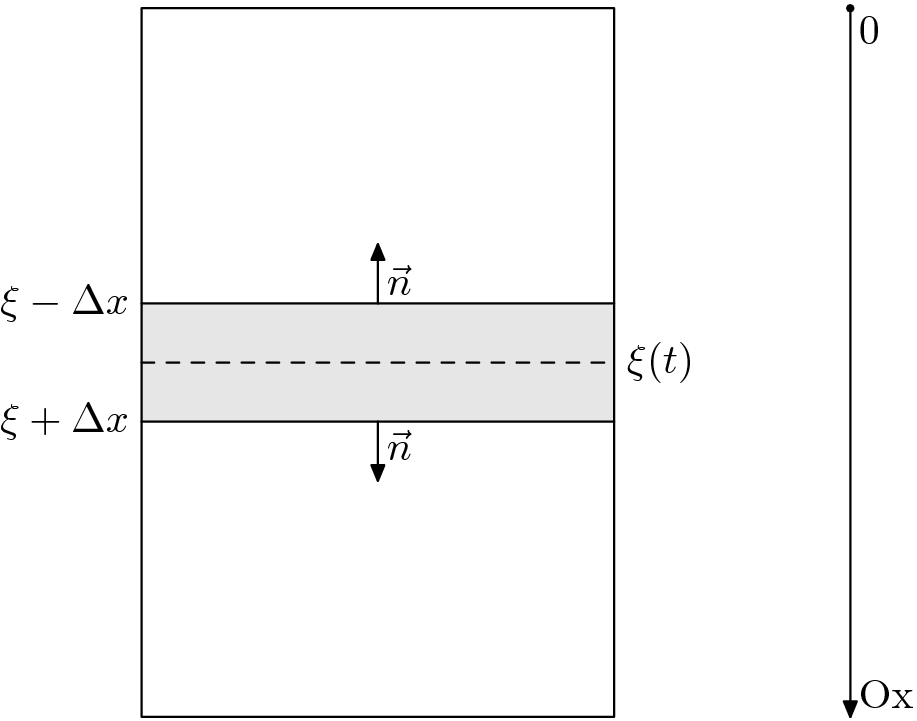
\includegraphics[width=.5\textwidth]{img/7-1.png}
\end{figure}

Отримаємо рівняння теплового балансу для нескінченно малого об'єму розплавленого металу, який знаходиться між перерізами $x$ та $x + \Delta x$ за проміжок часу від $t$ до $t + \Delta t$. \medskip

Обчислимо кількість тепла, яка необхідна для зміни температури у виділеному елементарному об'ємі від значення $u(x, t)$ до значення $u(x, t + \Delta t)$. Кількість тепла, що міститься в виділеному об'ємі в момент часу $t$ можна обчислити за формулою
\begin{equation}
	\diff Q(t) = c_l \cdot \rho_l \cdot S \cdot \Delta x \cdot u(x, t).
\end{equation}

Аналогічно для моменту часу $t + \Delta t$ кількість тепла дорівнює
\begin{equation}
	\diff Q(t + \Delta t) = c_l \cdot \rho_l \cdot S \cdot \Delta x \cdot u(x, t + \Delta t).
\end{equation}

При цьому нехтуємо, зміною температури по просторовій змінній у середині елементарного об'єму. Тоді кількість тепла, необхідна для зміни температури всередині об'єму дорівнює:
\begin{equation}
	\Delta Q(t, t + \Delta t) = c_l \cdot \rho_l \cdot S \cdot \Delta x \cdot (u(x, t + \Delta t) - u(x, t)).
\end{equation}

Ця зміна може відбуватися за рахунок теплових потоків, через перерізи $x$ та $x + \Delta x$. Підрахуємо кількість тепла, яка поступає всередину тіла через переріз $x + \Delta x$ за час $\Delta t$:
\begin{equation}
	\diff Q(x + \Delta x) = k_l \cdot \frac{\partial u(x + \Delta x, t)}{\partial \vec n} \cdot S \cdot \Delta t k_l \cdot \frac{\partial u(x + \Delta x, t)}{\partial x} \cdot S \cdot \Delta t
\end{equation} 
  
Напрям нормалі $\vec n$ в цьому перерізі співпадає з напрямом вісі $Ox$. \medskip

Кількість тепла, яка поступає всередину тіла через переріз $x$ за час $\Delta t$ можна записати у вигляді:
\begin{equation}
	\diff Q(x) = k_l \cdot \frac{\partial u(x, t)}{\partial \vec n} \cdot S \cdot \Delta t = - k_l \cdot \frac{\partial u(x + \Delta x, t)}{\partial x} \cdot S \cdot \Delta t
\end{equation} 

Таким чином можна скласти рівняння теплового балансу:
\begin{equation}
	\diff Q(t, t + \Delta t) = \diff Q(x + \Delta x) + \diff Q(x).
\end{equation}
 
Або після підстановки відповідних значень поділених на $\Delta x \cdot \Delta t \cdot S$ отримаємо:
\begin{equation}
	\frac{c_l \cdot \rho_l \cdot (u(x, t + \Delta t) - u(x, t))}{\Delta t} = k_l \cdot \left( \frac{\partial u(x + \Delta x, t)}{\partial x} - \frac{\partial u(x, t)}{\partial x} \right) \cdot \frac{1}{\Delta x}.
\end{equation}
  
Після граничного переходу коли $\Delta x$ та $\Delta t$ прямують до нуля, отримаємо диференціальне рівняння:
\begin{equation}
	c_l \cdot \rho_l \cdot \frac{\partial u(x, t)}{\partial t} = k_l \cdot \frac{\partial^2 u(x, t)}{\partial x^2},
\end{equation}
де $\xi(t) < x < L$, $t > t_0$. \medskip

Аналогічні міркування дозволяють отримати рівняння для твердої фази:
\begin{equation}
	c_s \cdot \rho_s \cdot \frac{\partial u(x, t)}{\partial t} = k_s \cdot \frac{\partial^2 u(x, t)}{\partial x^2},
\end{equation}
де $0 < x < \xi(t)$, $t > t_0$. \medskip

\begin{definition}[співвідношення на границі розділу фаз]
	Температура при переході через границю розділу фаз повинна змінюватись неперервно і співпадати з температурою плавлення металу, тобто повинно виконуватись настуну співвідношення:
	\begin{equation}
		u(\xi(t) - 0, t) = t(\xi(t) + 0, t) = U_{melt},
	\end{equation}
	яке називається \it{співвідношенням на границі розділу фаз}.
\end{definition}

Отримаємо рівняння теплового балансу для елементарного об'єму обмеженого перерізами $\xi(t) - \Delta x$ та  $\xi(t) + \Delta x$. \medskip

За час $\Delta t$ затвердіє об'єм металу рівний
\begin{equation}
	(\xi(t + \Delta t) - \xi(t)) \cdot S.
\end{equation}

При цьому буде виділено кількість тепла рівна
\begin{equation}
	\diff Q_{melt} = (\xi(t + \Delta t) - \xi(t)) \cdot S \cdot \lambda \cdot \rho_s.
\end{equation}

Кількість тепла, яка надійде всередину об'єму за рахунок теплових потоків через відповідні перерізи за час $\Delta t$ може бути записана у вигляді:
\begin{equation}
	\Delta t \cdot S \cdot \left( k_l \cdot \frac{\partial u(\xi(t) + \Delta x, t)}{\partial x} - k_s \cdot \frac{\partial u(\xi(t) - \Delta x, t)}{\partial x}\right).
\end{equation}
 
Оскільки фазовий перехід відбувається при постійній температурі, то в околі границі розділу фаз $\xi(t)$ зміною температури по змінній $t$ можна нехтувати, в зв'язку з чим можна не враховувати кількість тепла, яка витрачається на зміну температури у виділеному елементарному об'ємі. \medskip

Рівняння теплового балансу для елементарного об'єму обмеженого перерізами $\xi(t) - \Delta x$ та $\xi(t) + \Delta x$ можна записати у вигляді:
\begin{multline}
	(\xi(t + \Delta t) - \xi(t)) \cdot S \cdot \lambda \cdot \rho_s = \\
	= \Delta t \cdot S \cdot \left( k_l \cdot \frac{\partial u(\xi(t) + \Delta x, t)}{\partial x} - k_s \cdot \frac{\partial u(\xi(t) - \Delta x, t)}{\partial x}\right)
\end{multline}

Поділивши обидві частини на $\Delta t$, скоротивши на $S$ і спрямувавши $\Delta x$, $\Delta t$ до нуля отримаємо співвідношення:
\begin{equation}
	\lambda \cdot \rho_s \cdot \frac{\partial \xi(t)}{\partial t} = k_l \cdot \frac{\partial u(\xi(t) + \Delta x, t)}{\partial x} - k_s \cdot \frac{\partial u(\xi(t) - \Delta x, t)}{\partial x}.
\end{equation}

\begin{definition}[внутрішніх граничних умов (умов спряження)]
	Останню умову 
	\begin{equation}
		\lambda \cdot \rho_s \cdot \frac{\partial \xi(t)}{\partial t} = k_l \cdot \frac{\partial u(\xi(t) + \Delta x, t)}{\partial x} - k_s \cdot \frac{\partial u(\xi(t) - \Delta x, t)}{\partial x}.
	\end{equation}
	разом із співвідношенням на границі розділу фаз називають \it{внутрішніми граничними умовами}, або \it{умовами спряження}.
\end{definition}

Запишемо початкові умови та умови на верхній та нижній основі циліндру:
\begin{itemize}
	\item В початковий момент часу задана температура розплавленого металу:
	\begin{equation}
		u(x, t_0) = U_0, \quad 0 < x < L.
	\end{equation}
	
	\item На верхній основі задана температура:
	\begin{equation}
		u(0, t) = U_1, \quad t > t_0.
	\end{equation}

	\item Нижня основа теплоізольована, тобто тепловий потік, який поступає всередину тіла дорівнює нулю:
	\begin{equation}
		\frac{\partial u(L, t)}{\partial x} = 0, \quad t > t_0.
	\end{equation}
	
	\item В початковий момент часу положення границі фазового переходу співпадає з верхньою основою циліндру: 
	\begin{equation}
		\xi(0) = 0.
	\end{equation}
\end{itemize}

Таким чином до моменту часу, коли весь метал затвердіє постановка задачі Стефана включає в себе диференційні рівняння, умови спряження, початкові умови та граничні умови. \medskip

\begin{remark}
	Після повного затвердіння металу, тобто коли $\xi(t_1) = L$, процес буде описуватись звичайним рівнянням теплообміну для $t > t_1$ з граничними умовами
	\begin{align}
		u(0, t) &= U_1, \\
		\frac{\partial u(L, t)}{\partial x} &= 0,
	\end{align}
	та початковою температурою $u(x, t_1)$.
\end{remark}

\end{document}
